\documentclass{article}
%
%
%
%
\usepackage{iclr2025_conference}
\usepackage{graphicx}
%

\usepackage{algorithm}
\usepackage{algpseudocode}

\usepackage[utf8]{inputenc} %

\usepackage{indentfirst,csquotes}
\usepackage{subfigure}
%
%
%
%

%
%
\def\withnotes{0}
\def\withcolors{0}
\ifnum\withnotes=1
\newcommand{\theertha}[1]{{\color{red}{theertha: #1}}}
\newcommand{\ahmad}[1]{{\color{cyan}{ahmad: #1}}}
\newcommand{\ziteng}[1]{{\color{blue}{ziteng: #1}}}
\newcommand{\ananth}[1]{{\color{green}{ananth: #1}}}
\newcommand{\fprost}[1]{{\color{yellow}{fprost: #1}}}
\newcommand{\jb}[1]{{\color{brown}{JB: #1}}}
\newcommand{\je}[1]{{\color{teal}{JE: #1}}}
\else
\newcommand{\theertha}[1]{}
\newcommand{\ahmad}[1]{}
\newcommand{\ziteng}[1]{}
\newcommand{\ananth}[1]{}
\newcommand{\fprost}[1]{}
\newcommand{\jb}[1]{{}}
\newcommand{\je}[1]{{}}
\fi
\ifnum\withcolors=1
\newcommand{\znew}[1]{{\color{purple}{#1}}}
\else
\newcommand{\znew}[1]{{{#1}}}
\fi

\newcommand{\p}{\pi_{\text{sft}}}
\newcommand{\sft}{\text{sft}}
\newcommand{\ro}{\text{ro}}
\newcommand{\bilevel}{\text{bilevel}}
\newcommand{\multitask}{\text{multi-task}}
%
%
%
%
%


%
%

\iclrfinalcopy
\usepackage{bm}
\usepackage{bbm}
\newcommand{\mc}{\mathcal}
\newcommand{\by}{{\bm{y}}}
\newcommand{\bx}{{\bm{x}}}
\newcommand{\bz}{{\bm{z}}}
\newcommand{\bX}{{\bm{X}}}
\newcommand{\bY}{{\bm{Y}}}
\newcommand{\bcX}{{\bm{\mathcal{X}}}}
\newcommand{\bcY}{{\bm{\mathcal{Y}}}}
\newcommand{\dd}{{\rm d}}
\newcommand{\cR}{\mathcal{R}}
\newcommand{\calr}{\hat{\qt}}
\newcommand{\tr}{\cR}
\newcommand{\reg}{\beta}
\newcommand{\idc}[1]{\mathbbm{1} \left\{ #1\right\}}
\newcommand{\E}{\mathbb{E}}
\newcommand{\KL}{D_{\text{KL}}}
\newcommand{\TV}{{d_{\rm TV}}}
\newcommand{\bphi}{\bm{\phi}}
\newcommand{\lR}{\log \hspace{-0.03in}\mc{R}}
\newcommand{\calp}{g_{\pp}}

\newcommand{\pp}{T}
%
\usepackage[colorlinks,citecolor=blue,bookmarks=true]{hyperref}       %
\usepackage{url}            %
\usepackage{booktabs}       %
\usepackage{amsfonts}       %
\usepackage{nicefrac}       %
\usepackage{microtype}      %
\usepackage{xcolor}         %

\usepackage{amsmath, amsthm}
\usepackage{enumitem}
%
\usepackage{color}
\usepackage{graphics}
\usepackage{graphicx}

\usepackage[capitalise]{cleveref}
\newcommand{\logr}{\mc{R}}
\newcommand{\Paren}[1]{\left(#1\right)}

\newcommand{\N}{{N}}
\renewcommand{\p}{{p}}
\renewcommand{\P}{{P}}
\renewcommand{\wr}{\mathbb{W}_{\op, \bp}} %
\newcommand{\bp}{{\pi_{\rm ref}}} %
%
\newcommand{\op}{\pi} %
\newcommand{\qt}{\mathcal{C}}
\newcommand{\iapo}{\texttt{InfAlign}\xspace}
\newcommand{\ctrl}{\texttt{CTRL}\xspace}

\newcommand{\kl}{\text{KL}}

\newcommand{\bon}{{\pi_{\N,r}}} %
\newcommand{\car}{\mathcal{C}} %
%
\newtheorem{theorem}{Theorem}
\newtheorem{lemma}{Lemma}
\newtheorem{corollary}{Corollary}
\newtheorem{definition}{Definition}
\newtheorem{prop}{Proposition}
\newcommand{\RR}{\mathbb{R}}

\newcommand{\bofn}{\texttt{BoN}\xspace}
\newcommand{\wofn}{\texttt{WoN}\xspace}


\usepackage{xspace}
\newcommand{\ie}{i.e.\@\xspace}
\newcommand{\aka}{a.k.a.\@\xspace}
\newcommand{\eg}{e.g.\@\xspace}
\newcommand{\etal}{et al.\@\xspace}
\newcommand{\wrt}{w.r.t.\@\xspace}
\newcommand{\iid}{i.i.d.\xspace}
\newcommand{\cL}{\mathcal{L}}
\makeatletter
\newcommand{\specificthanks}[1]{\@fnsymbol{#1}}
\makeatother
\begin{document}
\title{InfAlign: Inference-aware language model alignment}
%
%
%
%
%
%
%


%
%
%
%
%
%
%
%
%

\author{\small Ananth Balashankar\thanks{Equal contribution.}\hspace{0.06in}$^1$\quad
Ziteng Sun$^{\specificthanks{1} 2}$ \quad Jonathan Berant$^{1}$\quad Jacob Eisenstein$^{1}$ \vspace{0.05in}\\
%
%
%
\bf \small Michael Collins$^1$ \quad Adrian Hutter$^1$ \quad  
Jong Lee$^1$ \quad 
Chirag Nagpal$^2$ \vspace{0.05in}\\
\bf \small
Flavien Prost$^1$  \quad 
 Aradhana Sinha$^1$ \quad
Ananda Theertha Suresh$^{2}$ \vspace{0.05in}\\
\bf \small 
Ahmad Beirami$^{1}$\\~\\
\small $^1$Google DeepMind \quad \quad \quad\quad $^2$Google Research}

%
%
%
%
%
%
%
%
%
%
%
%
%
%

\maketitle
%
%
%
%
%
%
\begin{abstract}
%
    Language model alignment has become a critical step in training modern generative language models.
    The goal of alignment is  to finetune a reference model %
    such that the {\em win rate} 
   of a sample from the aligned model over a sample from the reference model is high, subject to a KL divergence constraint.
    Today, we are increasingly using inference-time algorithms (e.g., Best-of-N, controlled decoding, tree search) to decode from language models rather than standard sampling. %
    However, the alignment objective does not capture such inference-time decoding procedures. We show that the existing alignment framework is sub-optimal in view of such inference-time methods. We then modify the alignment objective and propose a framework for inference-aware alignment (\iapo).
    We prove that for any inference-time decoding algorithm, the optimal solution that optimizes the {\em inference-time win rate} of the aligned policy against the reference policy is the solution to the typical RLHF problem with a {\em transformation of the reward}.
    This motivates us to provide the KL-regularized {calibrate-and-transform RL (\ctrl)} algorithm to solve this problem,
    which involves a reward calibration step and a KL-regularized reward maximization step with a transformation of the calibrated reward.
        We particularize our study to two important inference-time strategies: best-of-$N$ sampling %
    and best-of-$N$ jailbreaking, where $N$ responses are sampled from the model and the one with the highest or lowest reward is selected. We propose specific transformations for these inference-time strategies and demonstrate that our framework offers significant improvements over existing state-of-the-art methods for language model alignment. Empirically, we outperform state-of-the-art methods that are designed without taking inference-time decoding into consideration by 8-12\% and 4-9\% on inference-time win rates over the Anthropic helpfulness and harmlessness dialog benchmark datasets. 
    %
    %
\end{abstract}

\section{Introduction} \label{sec:intro}
Aligning generative language models (LMs) through KL-regularized reinforcement learning (KL-RL) is a widely adopted framework for finetuning a generative language model to improve a reward (e.g., safety or quality). Solving KL-RL generally entails training a reward model, and then using an RL solver~\citep{christiano2017deep, stiennon2020learning, ouyang2022training}. Other ways of solving KL-RL include variants of direct preference optimization~\citep{rafailov2024direct, azar2023general}, reward model distillation~\citep{fisch2024robust}, and Best-of-$N$ distillation~\citep{yang2024asymptotics, gui2024bonbonalignmentlargelanguage, amini2024variationalbestofnalignment, sessa2024bondaligningllmsbestofn}.
The success of the KL-RL framework is typically measured through the win rate of the aligned model over the reference model for a given task, which captures how often a sample drawn from the aligned model wins against a sample drawn from the base model using a judge for that task. 

However, rarely is the aligned model used as is at inference time; instead an {\em inference-time procedure} is typically used to accomplish a task. For example, it is customary to perform one or more of the following simple or complex procedures at decoding: best-of-$N$ sampling ~\citep{nakano2022webgptbrowserassistedquestionansweringhuman, beirami2024theoretical}, best-of-$N$  jailbreaking~\citep{hughes2024bestofnjailbreaking}, chain-of-thought reasoning~\citep{wei2022chain, o1}, and self consistency~\citep{self-consistency} (see \cref{sec:related} for more).
%
This creates a discrepancy between the inference-time decoding procedure and the training KL-RL objective, %
%
which is to maximize the expectation of a function of reward (e.g., win rate) of a sample from the aligned model against that of the base model.

%

In this paper, we address the following question: Given a known inference-time procedure, can we align a model to optimize for the {\em inference-time win rate} against the reference model, where inference-time win rate entails obtaining a response from each model through the \emph{inference-time procedure} and counting which sample wins? %
While directly optimizing the inference-time win rate seems intractable,
%
we show that the optimal solution is captured via a family of optimization objectives, which we call the {\em inference-aware alignment} (\iapo) framework. 
%
We further prove that for a $\delta$-bound language model, where the likelihood of all outcomes are upper-bounded by $\delta,$ as $\delta \to 0,$ the solution could be obtained by solving KL-RL with a specific transformation of the reward (\cref{thm:exisitence_informal}). Therefore, the challenge of optimizing for inference-time win rate can be captured by designing a reward transformation that is suited to the specific inference-time procedure, and solving KL-RL using existing optimization algorithms like PPO \citep{schulman2017proximal}.


%
%

We particularize the study of \iapo to two simple yet popular inference-time strategies: Best-of-$N$ (\bofn) sampling~\citep{nakano2022webgptbrowserassistedquestionansweringhuman, beirami2024theoretical} and Best-of-$N$ jailbreaking \citep{hughes2024best}, which we call Worst-of-$N$ (\wofn) since the defender may assume that the attacker is choosing the worst outcome of $N$ samples. %
Despite their simplicity, \bofn is extremely effective, and even known to be an effective procedure for inference-time alignment~\citep{beirami2024theoretical, gui2024bonbonalignmentlargelanguage, mudgal2023controlled}.  \wofn is a popular safety evaluation strategy often adopted to evaluate the ability to jailbreak foundation models \citep{yohsua2024international, pair, souly2024strongreject, hughes2024bestofnjailbreaking}. Hence, there is both theoretical and practical motivation for training to optimize inference-time \bofn and \wofn win rates. For these procedures, we solve \iapo for different values of $N$ in the limit of infinitely expressive language models. We also show that exponential reward transformation is almost optimal for these strategies. We further show that the win rate optimal solution to KL-RL without reward transformation leads to suboptimal policies for inference-time win rate.

Motivated by our theoretical findings, we propose a practical solver for \iapo, called Calibrate-and-Transform Reinforcement Learning (\ctrl), which adopts a three-step approach: (1) we first {\it calibrate} the scores of the reward model with respect to responses sampled per-prompt by the reference model; (2) we then adopt a suitable {\it transformation} of the calibrated scores for a given inference-time procedure; and (3) we solve the KL-RL problem (e.g., using PPO).

%


We apply \ctrl to the Anthropic helpfulness and harmlessness dataset~\citep{bai2022training} for optimizing \bofn helpfulness and \wofn harmlessness with various values of $N.$  We show that the (close-to-optimal) exponential reward transformations that were derived theoretically on idealized distributions transfer to real-world tasks -- outperforming various KL-RL solvers at inference-time win rate. Finally, we also show \ctrl (without any reward transformation) is a strong baseline for optimizing the standard win rate vs KL trade-off against various methods.
%
%

%
%

Our contributions are as follows:
%
%
\begin{itemize}
   \item We propose a framework for inference-aware language model alignment (\iapo) that captures the optimal solution to optimizing win rate in view of any well-behaving inference-time procedure. Theoretically, we show that this framework satisfies a coupled-transformed reward/policy optimization objective which lends itself to iterative optimization for a large class of inference-time procedures (see Section \ref{sec:calibration}).
    %
    %
    \item Motivated by our theoretical findings, we propose a practical solver, calibrate-and-transform RL (\ctrl) for \iapo, which consists of an offline reward calibration and transformation step prior to applying the regular KL-RL framework. For two popular inference-time procedures, namely optimizing Best-of-$N$ (\bofn) sampling and preventing Best-of-$N$ jailbreaking (\wofn), we derive the conditions for optimal theoretical solutions to alignment in a toy setting. Somewhat surprisingly, for \bofn and \wofn, the optimal solution is independent of the base policy and the reward model, which leads to an iterative optimization approach that can be computed offline (see \cref{sec:ctrl} and \cref{sec:implementation}).
    \item 
    %
    Empirically, we show on Anthropic dialog helpfulness and harmlessness datasets that \ctrl with identity reward transformation achieves competitive performance compared to a variety of SOTA methods for optimizing standard win rate~\citep{gui2024bonbonalignmentlargelanguage, amini2024variationalbestofnalignment, sessa2024bondaligningllmsbestofn, azar2023general, rafailov2024direct}, and produces
    %
    %
    better inference-time win rate vs KL tradeoffs by 8-12\% for \bofn and 4-9\% for \wofn inference-time procedures respectively (see  \cref{sec:results}).
    %
\end{itemize}






\section{Problem setup} \label{sec:setup}
%

We consider a generative language model that produces a response conditioned on an input prompt. %
%
Given a prompt $\bx$, \eg, $\bx = \textit{What is a large language model?},$ a generative language model $\bp$ returns a response $\by$,  which is sampled according to the distribution $\bp(\cdot \mid \bx)$. We use $\bcX$ and $\bcY$ to denote the space of possible inputs and outputs, respectively. Throughout the paper, we refer to the conditional distribution $\pi(\cdot \mid \bx)$ introduced by the language model as a policy, and assume $\bp$ is a fixed base policy, \eg, obtained from supervised finetuning. We will often use the notation $\pi(\by \mid \bx) \propto f(\by)$ for some $f: \bcY \rightarrow \RR_+$ to denote the conditional distribution $\pi(\by \mid \bx) = f(\by)/(\sum_{\by}f(\by)\dd\by)$ obtained after normalization.
%
%

\paragraph{Alignment of language models.} Let $r: \bcX \times \bcY \rightarrow \mathbb{R}$ be a reward function that assigns a scalar value to any (prompt, response) pair, e.g., a model trained side-by-side on human preferences. The reward determines the goodness of response $\by$ in context $\bx$. The goal of language model alignment is to construct an aligned distribution $\op$ that improves the reward of the response while being close to $\bp$. Below we introduce 
 \kl-regularized reinforcement learning (RL), a popular training-time alignment framework in the literature.

%
%
%
%
%
%
%
%
%
%
%
%
%
%
%
%
%
%
%
%
%
%
\begin{definition}[\kl-regularized RL framework] \label{def:kl_rl}
    Let $\beta > 0$ be a regularization parameter, the KL-regularized RL problem aims to maximize the pointwise expected reward with a KL regularizer
    %
    below: $\forall \bx,$
    \begin{equation}
    %
   \op^*_{r, \beta}(\cdot \mid \bx) = \arg \max_{\op} \left\{ \mathbb{E}_{\by \sim \op(\cdot \mid \bx)} \{r(\bx, \by)\} - \beta \KL(\op(\cdot \mid \bx) \| \bp(\cdot \mid \bx))\right\}.\footnote{%
    The solution to this optimization problem is unique~\citep{korbak2022rl,rafailov2024direct,yang2024asymptotics}. %
    } 
    \end{equation}
    %
    %
    %
    %
    %
    %
    %
    %
    %
    %
    %
%
%
%
%
\end{definition}

%
%
%
%
%
%
%
%


When evaluating an aligned policy, a common measure to use is the win rate over the base policy 
$\bp$. Let 
\[
    w_r(\by, \bz \mid \bx) := \idc{r(\bx, \by) > r(\bx, \bz)} +  \frac{1}{2}\idc{r(\bx, \by) = r(\bx, \bz)}
\]
be the win random variable under reward  $r$. 


\begin{definition}[Calibrated reward]
Let 
$\qt_{r, \pi}( \bx, \by)$ be the {\it calibrated reward} \footnote{The definition is similar to the cumulative density function of the reward $r(\bx, \by)$ under policy $\pi$ except for how ties are decided.} %
under policy $\pi$ defined below
%
%
%
\begin{equation}
    \qt_{r, \pi}(\bx, \by) :=  \mathbb{E}_{\bz \sim \pi(\cdot \mid \bx)} w_r(\by, \bz \mid \bx). \label{eqn:def_quantile}
\end{equation}
%
%
%
\label{def:calibrated-reward}
\end{definition}


The win rate is defined as following:
%

\begin{definition}[Win rate]\label{def:win_rate}
%
For any policy $\pi_1$ and $\pi_2$, we define win rate of policy $\pi_1$ over policy $\pi_2$ given prompt $\bx$, as measured by reward $r$ as follows:
\begin{equation} 
     W_r(\pi_1 \succ \pi_2 \mid \bx) := \E_{\by \sim \op_1(\cdot\mid \bx)} \qt_{r, \pi_2}(\bx, \by).
\end{equation}
%
%
%
%
%
%
%
\end{definition}


In this paper, for simplicity of the presentation and analysis, we assume that the language model is continuous, whose outcomes have infinitesimally small probabilities.
In other words, we assume $\bcY$ is a continuous set, which can be mapped to $[0, 1]$ through a CDF inverse transformation~\citep{Rosenblatt1952}, with the ordering determined by the reward of the outcomes from the smallest reward to the highest reward.
%
We also assume that $r$ assigns distinct rewards to different $\by$'s for a given $\bx$. 
These assumptions have been made in the past implicitly by~\cite{hilton2022measuring} to estimate the KL divergence of Best-of-$n$ policy, and by \cite{gui2024bonbonalignmentlargelanguage} to estimate its win rate and characterize the KL divergence and win rate of optimal policy for win rate vs KL divergence tradeoffs. While these assumptions lead to approximations when analyzing real-world distributions, the results derived under them are reasonably tight when the actual likelihood of the language model outcomes are small~\citep{beirami2024theoretical}. %
Note that we don't make any such assumptions when providing our algorithmic developments, and the experimental results.
%
%
%
%
%
%
%
Under these assumptions, we define the quantile mapping, which is the reverse of the calibrated reward mapping $\qt^{-1}$, satisfying $\forall u \in [0,1]$, %
$$\qt^{-1}_{r, \pi, \bx} (u) = \by_{u, \bx} \quad \text{where} \quad \qt_{r, \pi} (\by_{u, \bx} \mid \bx) = u.$$

\paragraph{Inference-time processing.} As mentioned earlier, in many cases we do not simply just sample from the language model. When decoding is done through an inference-time procedure, the obtained sample follows a transformed distribution that depends on the aligned policy and the inference-time procedure.
%
For example, when the inference-time procedure is \bofn from the base policy $\pi$, it can be shown that the final obtained sample is distributed proportional to $\pi(\by \mid \bx) \qt_{r, \pi}(\bx, \by)^{N-1}$~\cite[Lemma 1]{beirami2024theoretical}. In this work, we model inference-time processing as a procedure $\pp$ that maps $\pi$ to a distribution $\pp(\pi)$,
\[
    \pi \stackrel{T}{\longrightarrow} T(\pi).
\]
%
In these cases, it is customary to compare the models by considering the following inference-time win rate of the aligned policy $\pi$.
\begin{definition}[Inference-time win rate] \label{def:pp_wr}
Under inference-time processing $T$, the inference-time win rate of policy $\pi_1$ over $\pi_2$ is defined as %
\begin{equation} 
     W^\pp_r(\pi_1 \succ \pi_2 \mid \bx) := \E_{\by \sim \pp(\pi_1)(\cdot \mid \bx), \bz \sim \pp(\pi_2)(\cdot \mid \bx)} \left\{w_r(\by, \bz \mid \bx)\right\}.
\end{equation}
%
\end{definition}


%



With the above definitions at hand, the goal of the paper is solve the following KL-regularized inference-time win rate maximization problem.

\begin{definition}[Inference-time win rate KL-regularized RL problem]
Let $T$ be a given inference-time procedure and $\reg > 0.$ Then, the optimization problem for maximizing inference-time win rate is posed as %
%
\begin{align} \label{eqn:kl-constrained-ppwr}
  \max_\op \left\{ W^\pp_r(\op \succ \bp \mid \bx) -\reg \KL(\op(\cdot \mid \bx) \| \bp(\cdot | \bx))\right\}.
\end{align}
\label{def:kl-constrained-ppwr}
\end{definition}
Note that this formulation reduces to the IPO objective \citep[Equation (8)]{azar2023general} when $T$ is the identity transformation and extends it otherwise for an arbitrary inference-time procedure.\footnote{One question that arises is the role of the KL divergence regularizer in \cref{eqn:kl-constrained-ppwr}. We argue that the regularizer essentially enables multi-tasking between the SFT task and the RL task, which we formally prove for log-linear models in \cref{app:role-KL}.  In other words, the KL divergence regularizer enables to preserve the core capabilities of the model while acquiring a new one through the KL-RL process.}




%

%

%
%

%
%
%
%
%



%
%
%


%

\section{Reinforcement learning with reward transformation} \label{sec:calibration}
In this section, we propose a general framework for solving the language model alignment problem defined in \cref{def:kl-constrained-ppwr}. Our approach is based on designing a new reward function $\tr$ based on the reward model $r$, the inference-time procedure $T$, and the base policy $\bp$, such that solving the KL-regularized RL problem (\cref{def:kl_rl}) with the transformed reward $\tr$ leads to an almost optimal solution to \cref{eqn:kl-constrained-ppwr}. More precisely, %
the aligned policy is the solution to the following optimization problem:
%
\begin{equation} \label{eqn:kl-rl-tr}
    \max_\pi \mathbb{E}_{\bx \sim \mu, \by \sim \op(\cdot \mid \bx)} \{\tr_{r, \bp, T}(\bx, \by) - \reg \KL(\op(\cdot \mid \bx) \| \bp(\cdot \mid \bx))\},
\end{equation}
where $\tr_{r, \bp, T}(\bx, \by)$ is a transformed reward function.
%
%
%
%
%
At first, it might not be immediately clear how \cref{eqn:kl-rl-tr} might help solve the problem in \cref{eqn:kl-constrained-ppwr}, however, we will show that for any inference-time procedure $T$, there exists a transformed reward $\tr$, which solves \cref{eqn:kl-constrained-ppwr}.
%


\begin{lemma} \label{thm:exisitence_informal}
For any base policy $\bp$, reward model $r$, inference-time procedure $T$, and $\reg > 0$, there exists a reward function $\tr_{r, \bp, T}$  such that the solution to \cref{eqn:kl-rl-tr} solves the optimization problem in \cref{eqn:kl-constrained-ppwr} (\cref{def:kl-constrained-ppwr}).
%
%
%
%
%
\end{lemma}

In general, such optimal reward transformation will depend on the base policy $\bp$, the post-hoc procedure $T$, and the reward function $r$. In the lemma below, we list the property that the reward transformation and the resulting optimal aligned policy must satisfy.
\begin{theorem}[Characterization of \iapo solution] \label{lem:coupled}
Assuming that $T$ is such that $\partial T(\pi)(\by_1\mid\bx)/ \partial \pi (\by_2\mid\bx)$ exists for all $\bx, \by_1, \by_2$, then we have the optimal transformed reward $\tr$ and the optimal policy $\pi^*$ in \cref{eqn:kl-constrained-ppwr} must satisfy the following coupled equations $\forall \bx, \by$
\begin{align}
\pi^*(\by|\bx) & \propto \bp(\by \mid \bx) e^{\frac{1}{\beta} \tr(\bx,\by)} \label{eqn:pi_update}\\
    \tr(\bx,\by) &=  \frac{\partial  }{\partial \pi(\by \mid \bx)}W^\pp_r(\pi \succ \bp \mid \bx) \label{eqn:reward_update}
    \\ & 
    = \sum_{\bz} \qt_{r, T(\bp)}(\bx, \bz) \frac{\partial  }{\partial \pi(\by\mid \bx)}T(\pi)(\bz \mid\bx), \label{eqn:reward_expand}
\end{align}
where $\qt_{r, T(\bp)}(\bx , \bz) $ is the calibrated reward under the inference-time transformed policy.
\end{theorem}
%
%
%

Missing proofs are presented in \cref{app:proofs}. \cref{lem:coupled} naturally leads to an iterative EM-style algorithm that (I) updates $\pi$ with $\mc{R}$ fixed based on \cref{eqn:pi_update} and (II) updates $\mc{R}$ with $\pi$ fixed based on \cref{eqn:reward_expand} until convergence.  However, such algorithm suffers from two drawbacks: first, for general language models, it is inefficient/intractable to evaluate \cref{eqn:reward_expand} since it involves evaluating the policy on a large, or even infinite output space; second, it is unclear whether such an algorithm could lead to the optimal solution.

%

%
%


To find more efficient ways to design reward transformations, we examine the case when no inference-time procedure is performed. In this case, $T(\pi) = \pi$ and 
\[
    \frac{\partial  }{\partial \pi(\by\mid \bx)}T(\pi)(\bz \mid\bx) = \mathbbm{1}\left\{\bz = \by\right\}.
\]
\cref{eqn:reward_expand} will reduce to $ \tr(\bx,\by) =  \qt_{r, \bp}(\bx, \by)$, the CDF or calibrated reward under $\bp$. 
\begin{corollary} \label{cor:no_inference_procedure}
When no inference-time procedure is performed, \ie $\forall \pi, T(\pi) = \pi$, the solution to \cref{eqn:kl-rl-tr} with $\tr(\bx,\by) =  \qt_{r, \bp}(\bx, \by)$ is the solution to \cref{eqn:kl-constrained-ppwr}.
\end{corollary}

%
Note that the above corollary is also observed in \citet{azar2023general,gui2024bonbonalignmentlargelanguage}. Hence \cref{lem:coupled} can be viewed as a generalization of these results with general inference-time procedures.
The observation motivates us to  consider a family of reward transformations based on this calibrated reward,
%
%
%
described in the
next section. As we will see, for the class of \textit{calibrated} inference-time procedures (\cref{def:calibrated_transformation}), different transformations in such family could be efficiently evaluated through a toy language model, which enables the search for good or even optimal transformations.
%

%

%



\section{Towards solving \iapo} \label{sec:ctrl}

%

We first state a few properties of reward calibration in \cref{sec:reward_calibration}. Then, in \cref{sec:kl_rl_calibration}, we demonstrate how this approach enables efficient evaluations of different transformations for calibrated inference-time procedures. 
%
%
We will then use best-of-$N$ and worst-of-$N$ as examples of post-hoc procedures to demonstrate the effectiveness of such an approach in \cref{sec:bon_won}. Missing proofs in the section are presented in \cref{app:proofs}.

\subsection{Reward calibration}
\label{sec:reward_calibration}
%
%
%




%

%
%
%
%
%
%
%
%
%
%
%
%
%
Recall the definition of the calibrated reward in \cref{def:calibrated-reward}.
%
In this section, we assume that  $\car_{r, \bp}$ is already obtained and discuss methods to approximate $\car_{r, \bp}$ in \cref{sec:implementation}.
We state a few properties of $\car_{r, \bp}$ below. %
The first property states that reward calibration preserves the ordering of the reward. This implies that the win rate evaluated under the calibrated reward stays unchanged. %
\begin{lemma}[Calibration is a bounded monotone increasing transformation of reward] \label{lem:monotone}
We have $\car_{r, \bp}(\bx, \by) \in [0,1].$ Furthermore, we have for any $\by$ and $\bz$ \begin{equation}
    r(\bx, \by) \geq r(\bx, \bz) \implies \car_{r, \bp}(\bx, \by) \geq \car_{r, \bp}(\bx, \bz)
\end{equation}
\end{lemma}

%

Moreover, we have that $\car_{r, \bp}$ is a canonical transformation of reward, and is invariant under all monotone increasing transformations of the reward function, stated below.
\begin{lemma}[The calibrated reward is invariant under monotone increasing transformations of reward]
Let $m: \mathbb{R} \to \mathbb{R}$ be any monotonic increasing function. Then,
\begin{equation}
    \car_{m(r), \bp} = \car_{r, \bp}.
\end{equation}
In particular, this also immediately implies that $\car_{\car_{r, \bp}, \bp} = \car_{r, \bp}.$
\label{lem:canonical}
\end{lemma}
This property is useful since as long as the learned reward model $r$ can capture relative human preference between pairs, the calibration of $r$ will be the same. Hence $\car$ is more robust to the learning process of $r$.

The next property shows that the calibration operation allows us to transform the distribution of the reward under the base policy to a uniform distribution over $[0, 1]$ regardless of the base policy $\bp$ and the reward model $r$.
\begin{lemma} \label{lem:reward_uniform}
If $\pi$ is a continuous language model, let $\by$ be sampled from $\bp(\cdot \mid \bx)$, then we have $\forall \bx$,
\[
    \car_{r, \bp}(\bx, \by) \sim {\rm Unif}([0, 1]).
\]
%
%
%
%
\end{lemma}

The lemma provides us a simple, unified view of the output from a language model through the space of calibrated reward, which is independent from the base policy, and the reward model.%
%
%
%
%
%

%
\subsection{KL-regularized RL with the calibrated reward}  \label{sec:kl_rl_calibration}

Next we discuss how the calibrated reward can be used in KL-regularized reinforcement learning. As \cref{lem:reward_uniform} suggests, after calibration, the reward distribution of the outputs from the base policy is independent from the reward model and the base policy itself. This allows us to design a transformation function  $\Phi$, focusing only on the inference-time procedure $T$, 
to be applied on top of the calibrated reward function, independent of $\bp$ and $r$. %

%
More precisely, let $\Phi: [0, 1] \rightarrow \RR $ be a transformation function, we propose the following reward function 
%
%
 \begin{equation} \label{eqn:transformed_reward}
   \cR_\Phi(\bx, \by) = \Phi(\car_{r, \bp}(\by\mid \bx)),
\end{equation}
and we would like the aligned policy to be the solution to the KL-regularized RL problem defined in \cref{def:kl_rl} with reward $\cR_\Phi(\bx, \by)$,
\begin{equation} \label{eqn:transformed_klrl}
    \op^*_{\cR_\Phi, \reg}(\cdot \mid \bx) = \arg \max_\op \mathbb{E}_{\by \sim \op(\cdot \mid \bx)} \{\cR_\Phi(\bx, \by)\} - \reg \KL(\op(\cdot \mid \bx) \| \bp(\cdot \mid \bx)).
\end{equation}
%
%
%
%
%

%
\paragraph{Inference-aware reward transformation.} For a given inference-time procedure $T$, our goal is to derive or design a suitable transformation $\Phi$, such that the solution leads to a good or even optimal trade-off between the inference-time win rate $W^T$ and the KL divergence  from the base policy.

\paragraph{Standard win rate (no inference-time procedure).} When no inference-time procedure is employed (i.e., $T$ is the identity mapping), $W^T$ reduces to the standard win rate. Setting $\Phi$ to be the identity transformation leads to the optimal win rate vs KL trade-off curve by noting that
\[
    \mathbb{E}_{\by \sim \op(\cdot \mid \bx)} \{\car_{r, \bp}(\bx, \by)\} 
    %
    = W_r(\pi \succ \bp \mid \bx).
\]
In this case, \cref{eqn:transformed_klrl} will be the same as the alignment objective of \citet{azar2023general}. Moreover, it can also be shown that when $\Phi(\cdot) = \log(\cdot)$, the solution $ \op^*_{\cR_\Phi, \reg}$ recovers the popular best-of-$N$ distillation objective, which has been studied in a recent line of works \citep{gui2024bonbonalignmentlargelanguage, amini2024variationalbestofnalignment,sessa2024bondaligningllmsbestofn}, and shown to be nearly win rate optimal~\citep{yang2024asymptotics, gui2024bonbonalignmentlargelanguage}.
%
%
We also note that while these methods lead to similar optimization objectives, the algorithmic approaches to solve the problems are different. In \cref{sec:implementation}, we will discuss a unified algorithm to solve \cref{eqn:transformed_klrl} for general $\Phi$. In \cref{sec:results}, we compare the results for $\Phi$ set to the identity mapping with the abovementioned baseline approaches.

We consider a family of inference-time procedures that only depend on the calibrated reward of the outputs, which we term \textit{calibrated procedures}, and discuss how to design a suitable $\Phi$ for this family of transformations. We first define \textit{calibrated procedures} below.

\begin{definition}[Calibrated inference-time procedure]\label{def:calibrated_transformation}
An inference-time procedure $T$ is called a \emph{calibrated procedure} if there exists a mapping function $\calp: [0, 1] \rightarrow \RR$ such that for any $\pi$, $r$, and $\bx, \by$, we have
\[
    T(\pi)(\by \mid \bx) \propto \pi(\by \mid \bx) \cdot \calp(\qt_{r, \pi} (\bx, \by)).
\]
\end{definition}
%

Our next result shows that for calibrated inference-time procedures, the aligned policy from solving \cref{eqn:transformed_klrl} has a win rate and KL divergence independent of the base policy and reward function.
\begin{theorem}[Model-agnostic property of calibrated inference-time procedures, informal version of \cref{thm:calibrated_procedure_extended}] \label{thm:calibrated_procedure}
If $T$ is a calibrated inference-time procedure, for any continuous language model $\pi$, $\reg > 0$ and reward transformation function $\Phi$,  we have that both $W^T_r(\op^*_{\cR_{\Phi}, \reg} \succ \bp \mid \bx)$ and $\KL(\op^*_{\cR_{\Phi}, \reg} \| \bp)$ are independent of $r$ and $\bp$.
\end{theorem}

%
%
%


%
The above theorem allows us to evaluate a transformation $\Phi$ by focusing on simple continuous language models that are easy to compute and simulate. In the next section, we will use two popular inference-time procedures, best-of-$N$ and worst-of-$N$, as examples to demonstrate how the theorem enables us to 
efficiently evaluate the inference-time win rate vs KL divergence tradeoff curve for different $\Phi$ functions, which could be used to find a suitable transformation $\Phi$ in practical scenarios.

%

%
%
%
%
%
%
%
%
%
%
%

%
%

%


%

%

\subsection{Finding better transformations for \bofn and \wofn} \label{sec:bon_won}

%
In this section, we focus on the following two inference-time procedures.
%

\noindent \textbf{Best-of-$N$ inference-time procedure (\bofn)}. During inference, $N$ \iid responses from a policy $\pi$ are generated, i.e., $\by_1, \ldots \by_N \sim \pi$. The final output is the one with the highest reward, i.e.,
    \[
        \by_{\bofn} = \arg \max_{\by \in  \{ \by_1, \ldots \by_N\}}
 r(\bx, \by)    .
 \]
 
\noindent \textbf{Worst-of-$N$ inference-time procedure (\wofn).}  Let $\by_1, \ldots \by_N$ be $N$ \iid draws from policy $\pi$. The final output is the one with the lowest reward. i.e.,
\[
    \by_{\wofn} = \arg \min_{\by \in  \{ \by_1, \ldots \by_N\}}
 r(\bx, \by)    .
\]
%
%
The lemma below presents the distribution of outputs after the inference-time procedure is performed.
%
\begin{lemma} \label{lem:bofn_wofn}
For any $N$ and continuous language model $\pi$,
\[
    \bofn(\pi)(\by \mid \bx) \propto \pi(\by \mid \bx) \cdot \qt_{r, \pi}(\bx, \by)^{N-1}.
\]
\[
    \wofn(\pi)(\by \mid \bx) \propto \pi(\by \mid \bx)   \cdot  (1 - \qt_{r, \pi}(\bx, \by))^{N-1}.
\]
\end{lemma}
Note that the results for \bofn have already been derived previously~\citep{beirami2024theoretical,gui2024bonbonalignmentlargelanguage,amini2024variationalbestofnalignment}.
The lemma shows that these two inference-time procedures are calibrated procedures so that as claimed in \cref{thm:calibrated_procedure}, for the aligned policy, the inference-time win rate and KL divergence deviation from the base policy are independent of the base policy and reward model. Below we present the precise formula for these two procedures.

%

\begin{theorem}[Properties of \bofn and \wofn procedures] \label{thm:wr_kl_bon_won}
For any transformation function $\Phi$, the solution $\pi^*_{\tr_{\Phi}, \reg}$ to the KL-regularized RL problem defined in \cref{eqn:transformed_klrl} satisfies the followings: Let $F_{\Phi, \reg}(u)= \frac{\int_{0}^u e^{\Phi(u')/\reg} \dd u'}{\int_{0}^1 e^{\Phi(u')/\reg} \dd u'}$. Then the following hold true:
\begin{itemize}
    \item The best-of-$N$ win rate over the base policy satisfies for any $\bx$,
    \[
    W^{\bofn}_r(\pi^*_{\tr_{\Phi}, \reg} \succ \bp \mid \bx) = 1 - N \int_{0}^1 F_{\Phi, \reg}(u)^N u^{N-1} \dd u,
    \]
    \item The worst-of-$N$ win rate over the base policy satisfies for any $\bx$,
    \[
    W^{\wofn}_r(\pi^*_{\tr_{\Phi}, \reg} \succ \bp \mid \bx) =  N \int_{0}^1 \Paren{1 - F_{\Phi, \reg}(u) }^N (1-u)^{N-1} \dd u,
    \]
     \item The KL divergence between $\pi^*_{r_{\Phi}, \reg}$  and $\bp$ satisfies
%
%
%
    \begin{equation}\label{eqn:kl_div_2}
    \KL(\op^*_{\cR_{\Phi}, \reg} \| \bp) =
\frac{1}{\reg}  \frac{ \int_{0}^1 \Phi(u) e^{\Phi(u)/\reg} \dd u }{\int_{0}^1 e^{\Phi(u)/\reg} \dd u} - \log \Paren{\int_{0}^1 e^{\Phi(u)/\reg} \dd u}.
    \end{equation}
\end{itemize}
\end{theorem}

By varying $\reg$ in \cref{eqn:transformed_klrl}, we can obtain an alignment curve plotting the inference-time win rate and KL divergence deviation for different aligned policies. This allows us to compare the performance of different transformation functions $\Phi$.

In the rest of the section, we will consider different types of transformations, and analytically compute the alignment curves using \cref{thm:wr_kl_bon_won} by varying $\reg$, \ie, the plot of $(\KL(\pi^*_{r_{\Phi}, \reg} \| \bp), W^{\rm T}_r(\pi^*_{r_{\Phi}, \reg}) \succ \bp)$ for different $\reg$'s. The transformations we consider include  optimal transformations for standard win rate, exponential functions, and optimization-based transformations, described below.

\paragraph{Optimal reward transformations for standard win rate.} The identity mapping proposed by \citet{azar2023general} and the logarithmic mapping as used by \bofn distillation \citep{beirami2024theoretical,yang2024asymptotics,amini2024variationalbestofnalignment,sessa2024bondaligningllmsbestofn} are shown to be (almost) optimal for the standard win rate. We would like to understand whether they are still good candidates when inference-time procedures are considered.
%

%

%



%

%

\paragraph{Deriving an optimized reward transformation function.} %
For calibrated inference-time procedures like \bofn, and \wofn, due to \cref{thm:calibrated_procedure}, we have that the optimal reward transformation $\Phi$ is independent of the base policy. One can optimize for good $\Phi$'s using simple toy language models, and we have the following corollary.

\begin{corollary}  \label{cor:coupled_won}
 For any $\reg > 0$, the $\Phi$ that achieves the optimal \bofn win-rate vs.  KL tradeoff must satisfy the following pair of equations:
%
%
%
%
%
%
%
%
%
\begin{gather*}
    \Phi_{\bofn}(u) = -N^2 \int_u^1 F_{\pi}(v)^{N-1} v^{N-1} \dd v ,\\
    f(u) \propto e^\frac{\Phi_{\bofn}(u)}{\reg},
\end{gather*}
and for \wofn, it satisfies that
\begin{gather*}
    \Phi_{\wofn}(u)  =  -N^2 \int_u^1 (1-v)^{N-1} (1 - F_{\pi}(v))^{N-1} \dd v,\\
    f(u) \propto e^\frac{\Phi_{\wofn}(u)}{\reg}.
\end{gather*}
\end{corollary}
%
%
Hence one can find a transformation function based on finding the fixed point of the coupled equations in \cref{cor:coupled_won} through iterative updates.




\begin{figure}[t]
    \centering
    \includegraphics[width=.48\textwidth]{win-rate-vs-KL.png}\\
    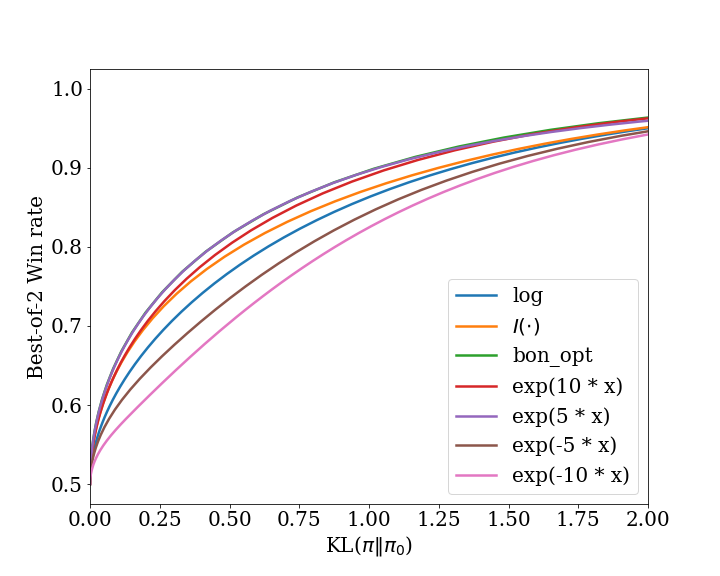
\includegraphics[width=.48\textwidth]{Best-of-2.png}
    \hfill
    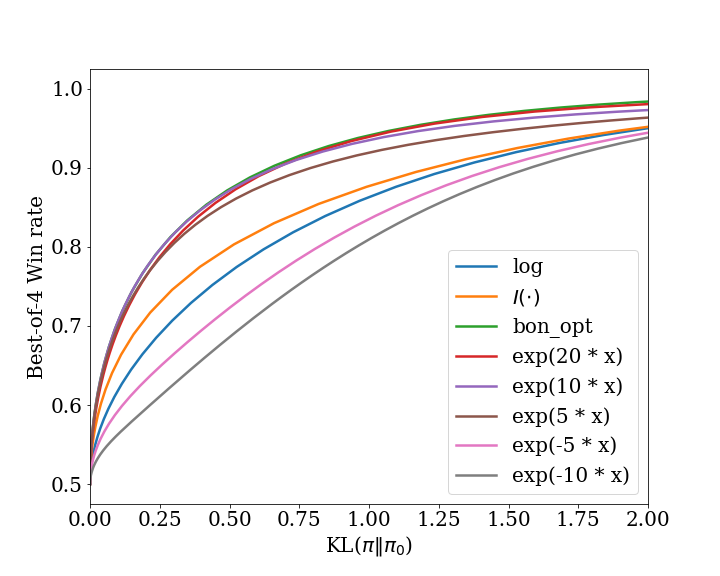
\includegraphics[width=.48\textwidth]{Best-of-4.png}
    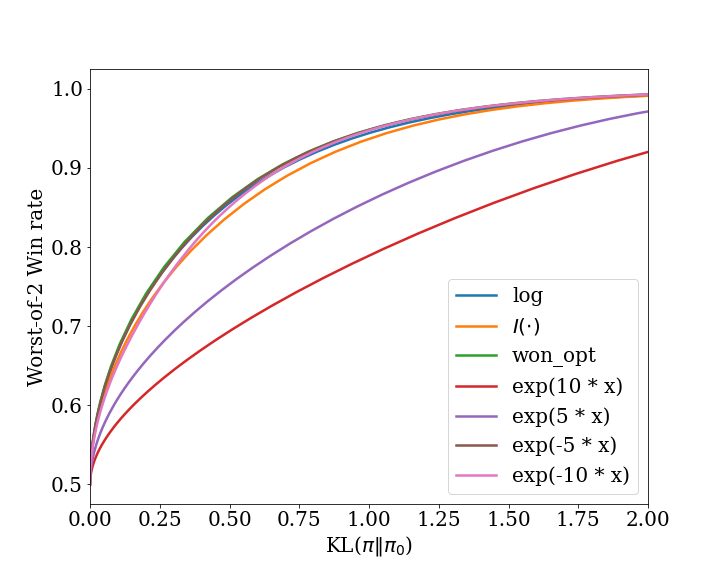
\includegraphics[width=.48\textwidth]{Worst-of-2.png}
    \hfill
    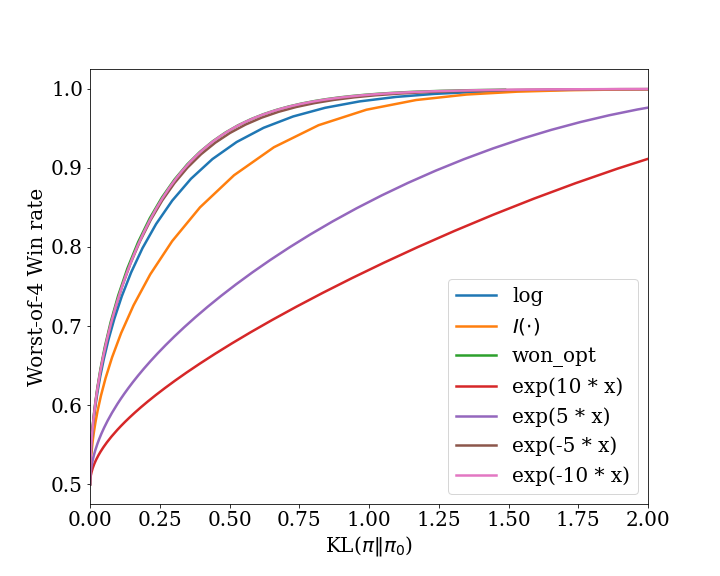
\includegraphics[width=.48\textwidth]{Worst-of-4.png}
    \caption{Best-of-$N$ and worst-of-$N$ win rate vs KL tradeoff curves for $N = 2, 4$ with different transformation functions. %
    }
    \label{fig:simulation}
\end{figure}


\paragraph{Exponential tilting for reward transformation.} In addition to deriving the optimized transformation, motivated by the exponential tilting of loss functions~\citep{li2021tilted, li2023tilted}, we consider the following exponential transformation: %
%
\begin{equation}
    \Phi_t(u) = \text{sign}(t) \cdot e^{t u},
\label{eqn:exp_transform}
\end{equation}
where $\text{sign}(t) = 1$ for $t\geq 0$ and $\text{sign}(t) = -1$ for $t<0.$
These exponential transformations are essentially helping to optimize different quantiles of the reward for different values of $t$~\citep{li2023tilted}. For a positive value of $t$, the exponential tilting transformation focuses on optimizing the high quantiles of the objective (calibrated reward) and indeed recovers the max function for a large positive $t$. Hence, we expect that positive values of $t$ help with \bofn inference-time procedure. On the other hand, for a negative value of $t$, the transformation is akin to optimizing the lower quantiles of the objective (calibrated reward), which makes it a suitable transformation for the \wofn inference-time procedure.



\paragraph{Results.} 
In \cref{fig:simulation}, we consider 
an ideal continuous language model and compare different alignment objectives on 
inference-time win rate vs KL divergence for three inference-time procedures: \{standard, \bofn, \wofn\}. The tradeoff curves are obtained by varying the strength of the regularizer, $\reg$.
The different objectives correspond to different transformations of the calibrated reward, which include (1) identity mapping  $\Phi =I(\cdot)$ (IPO); (2) logarithmic mapping $\Phi = \log$ (best-of-$N$ distillation); (3) exponential tilting $\Phi_t(\cdot)$ as defined in \cref{eqn:exp_transform}; (4) optimized transformation function by solving for fixed points in \cref{cor:coupled_won}.

In the first plot, we consider standard win rate. In this case, it is known that the IPO objective is win rate optimal. As can be seen, the logarithmic transformation (i.e., best-of-$N$ distillation) also achieves a nearly optimal win rate, which was already observed by~\citet{yang2024asymptotics, gui2024bonbonalignmentlargelanguage}. All other transformations are sub-optimal for standard win rate.

Next, we consider Best-of-$2$ and Best-of-$4$ win rate. Here, additionally we include \texttt{bon\_opt}, which is obtained by deriving the fixed point of \cref{cor:coupled_won}. As can be seen, the identity transformation is no longer optimal. The best tradeoffs are given by \texttt{bon\_opt}. We also observe that $\exp(5x)$ and $\exp(10x)$ are almost as good as \texttt{bon\_opt} for Best-of-$2$ and Best-of-$4,$ respectively. Moreover,the identity transformation and logarithmic transformation are sub-optimal in these cases, which shows that considering standard win rate as the only metric is not optimal when inference-time procedure is concerned.  We also observe that the behavior of identity transformation and logarithmic transformation is different in that the identity transformation gives better tradeoffs.

Finally, we consider Worst-of-$2$ and Worst-of-$4$ win rate. Again, it can be observed that \texttt{bon\_opt} gives the best tradeoffs for this inference-time procedure. Here, $\exp(-5x)$ and $\exp(-10x)$ are almost as good for Worst-of-$2$ and Worst-of-$4,$ respectively. We also observe that identity transformation and logarithmic transformation are sub-optimal in these cases and the logarithmic transformation gives better tradeoffs for \wofn compared to the identity transformation.


%
%
%
%

The above results demonstrate the importance of considering the inference-time procedure when performing alignment. We find that exponential transformation with different $t$'s are good for different inference-time procedures, which will be our focus in practical experiments.
%
Next, we will examine whether a good transformation that we found on the idealized continuous language model generalizes in the wild to real-world scenarios. Before moving on to the experiments, we will have to offer a practical algorithm for solving the inference-time KL-regularized RL optimization problem, which is the subject of the next section.

%



%


%
%
%
%
%
%
%
%




%
%
%
%
%
%
%

%
\section{\ctrl: Calibrate-and-Transform Reinforcement Learning} \label{sec:implementation}
%

%

In this section, we propose the \ctrl\ method, which is our proposed solver for the inference-time win rate optimization problem. Recall from the previous section that the proposed solution could be decomposed into three stages: {\em reward calibration} and {\em reward transformation} followed by the standard KL-RL solver. In the previous section, we highlighted the reward transformation. In the rest of this section, we focus on approximate empirical calibration. Combining it with reward transformation yields the final $\ctrl$ algorithm, given in Algorithm~\ref{alg2}.


%



%
%

%
%
%

%
%


\begin{algorithm}[ht]
\caption{\ctrl Algorithm for \bofn and \wofn} \label{alg2}
\begin{algorithmic}[1]
\Require Base policy $\bp$, (uncalibrated) reward model $r$, training prompts $\bx \in \mathcal{X}$, number of offline rollouts per prompt $m$. 
\State Compute approximate empirical calibration function $\widehat{\car}_{r, \bp} $ using Algorithm~\ref{alg1} with $m$ offline rollouts per prompt.
\State Transform calibrated reward using exponential function per  \cref{eqn:exp_transform} with $t>0$ for \bofn and $t < 0$ for \wofn.
\State Optimize KL-RL using calibrated and transformed reward per \cref{eqn:kl-rl-tr}.
\end{algorithmic}
\end{algorithm}



%
Consider {\em empirical calibration}, where we draw $K$ samples $\bz_1,\bz_2, ..., \bz_K$ from the reference model $\bp$ for each prompt $\bx$ in the RL training data. We then sort the rewards to all the responses $\{r(\bx, \bz_1), r(\bx, \bz_2),... r(\bx, \bz_K)\}$, and assign {\em empirical calibrated reward} scores during RLHF training for the prompt, response pair $(\bx, \by)$ as  
%
%
\begin{align}
    \widetilde{\car}_{r, \bp}(\bx, \by) = \frac{1}{K} \sum_{i=1, z_i \sim \bp}^K  \mathbbm{1} [r(\bx, \by) \geq r(\bx, \bz_i) ].
\end{align}
Ideally, as $K \rightarrow \infty$, the empirical calibrated reward would converge to the true calibrated reward, and may be used in the RL training objective through PPO \citep{schulman2017proximal}. However, this could be costly
%
as the exact computation of this calibrated reward requires us to sample and store $K$ reward scores per-prompt and per roll-out in the KL-RL solvers. 

Instead, we propose to {\em approximate} the calibration curve by scaling it with a step-wise function in the logarithmic domain. We do this by choosing $p$ anchor points $q_1, q_2,\ldots$, where at each of the quantiles $q_i \in (0,1)$ we achieve zero calibration error.
%
The algorithm for the simpler case ($p=1$, median) is given in Algorithm~\ref{alg1}. For larger values of $p$, the algorithm is given in Algorithm~\ref{app:algorithm} (\cref{sec:more_anchors}). 
%
%
%


%


%

\begin{algorithm}[ht]
\caption{Offline Approximate Calibration} \label{alg1}
\begin{algorithmic}[1]
\Require Base policy $\bp$, (uncalibrated) reward model $r$ with range $[0, 1]$, training prompts $\bx \in \mathcal{X}$, number of samples per prompt $m$. 
%
%
\ForAll{$\bx \in \mathcal{X}$}
\State Roll out $m$ i.i.d. samples from $\bp$ per training prompt $\bx$: $\bz_{j},\, j \in \{1...m\}$. %
%
%
%
\State $r_{\text{median}}(\bx) \leftarrow \text{median}(r(\bx, \bz_{1}), \ldots, r(\bx, \bz_{m}))$.
%
\EndFor
%
\State Define the calibrated reward function $\widehat{\car}_{r, \bp}: \mathcal{X} \times \mathcal{Y} \to [0, 1]$ as follows:
\begin{align*}
  \log \widehat{\car}_{r, \bp}(\bx, \by) =
  \log  r(\bx, \by) \cdot 
  \frac
  {
  \log 0.5 
  }
  {\log  r_{\text{median}}(\bx)  } .
\end{align*}
 \State \textbf{Output:} Calibrated reward function  $\widehat{\car}_{r, \bp}$ that assigns a calibrated reward for all prompts in the training set.
\end{algorithmic}
\end{algorithm}




%
%


%

%
%
%
%
%
%
%
%
%
%
%
%
%

%
%
%
%
%
%

%
%
%
%
%

%
%
%
%
%
%
%
%
%
%

%
%



%



%
%


%



%

%

%
%

%
%









\section{Experiment Results} \label{sec:results}


\subsection{Evaluation setup} \label{sec:evaluation}
\paragraph{Datasets.}
To train the reward models, we use the Anthropic Helpfulness and Harmlessness datasets \citep{bai2022training} which involve multi-turn dialogues between a human and a digital assistant. The preference datasets consist of
two responses for one context, and a label for the human preference for the response. We use the train split of the two datasets (44K examples for helpfulness and 42K for harmlessness) to train the uncalibrated and calibrated reward models -- separate reward models for each objective.

\paragraph{Model.}
The uncalibrated reward model is trained based on the Bradley-Terry pairwise objective \citep{raffel2020exploring}, and the calibration is done on the training-split of the RL training procedure by drawing samples from the reference model. The underlying model for both these rewards is the PaLM-2 S model \citep{anil2023PaLM}. The base reference policy model is a PaLM-2 S model that is fine-tuned (SFT) on the Anthropic dialog preferred responses. We then train the aligned policy model through KL-regularized Reinforcement Learning \citep{schulman2017proximal, bai2022training}. We compare against \texttt{uncalibrated} (a model trained with KL-RL using PPO and no further processing), \texttt{BoNBoN}~\citep{gui2024bonbonalignmentlargelanguage}, \texttt{Best-of-N}~\citep{nakano2022webgptbrowserassistedquestionansweringhuman, beirami2024theoretical}, \texttt{BonD}~\citep{sessa2024bondaligningllmsbestofn}, and \texttt{IPO}~\citep{azar2023general} as baselines.

\vspace{-.05in}
\paragraph{True rewards.} As evaluating using ground truth rewards in a pointwise manner based on human annotations can be expensive, we follow \cite{eisenstein2023helping, mudgal2023controlled} and perform automated evaluation using a larger PaLM-2 M model to compute \textit{true rewards}.

\vspace{-.05in}
\paragraph{Metrics.}
To measure improvement due to post-RL training, we report both the win rate and the \bofn and \wofn win rates, calculated after applying the respective inference-time procedures on the responses generated by the RL model against the base SFT model, along with the corresponding KL-divergence of the RL model with the SFT model. For each of the runs, we experiment with different KL-regularizer strengths ($\beta \in \{0.01, 0.02, \ldots , 0.09\}$) and obtain the Pareto-curve of the KL divergence vs \{standard, \bofn, \wofn\} win rate curves. 

%
\subsection{Reward models are typically miscalibrated}
We first validate our hypothesis that reward models used on real-world tasks are miscalibrated. We measure the miscalibration of the reward model trained on Anthropic helpfulness preference dataset by computing the scores of $100$ reference-policy responses for $10$ random prompts from training split. \theertha{ananth: for next iteration, regenerate figure 2 on test split.} We then sort the scores and compute the ranks corresponding to each of the responses and plot these values as a scatter plot in Figure~\ref{fig:1} (left). If the model were perfectly calibrated, the points for each prompt would lie on the line $y=x$. However, observe that for most prompts, the scatter plot deviates significantly from the $y=x$ line, and the extent of this deviation varies depending on the prompt.

We then measure the  Absolute Error (AE) between the reward scores and their corresponding ranks and  plot the cumulative distribution function (CDF) of the AE of the various calibration approximations in Figure~\ref{fig:1} (right). If the model is well-calibrated AE is zero always and hence the CDF reaches one at zero AE. We find that the reward scores (see legend named `identity') are not calibrated (mean AE: $0.22$)
%
and using fixed reward polynomial transformation functions like square-root, cube, square - do not reduce the calibration error (mean AE $> 0.15$). However, using a per-prompt quantile-based reward calibration, see legend named `quantile') significantly reduces the calibration error (mean AE: $0.02$).

\begin{figure}
    \centering
     \begin{subfigure}
    {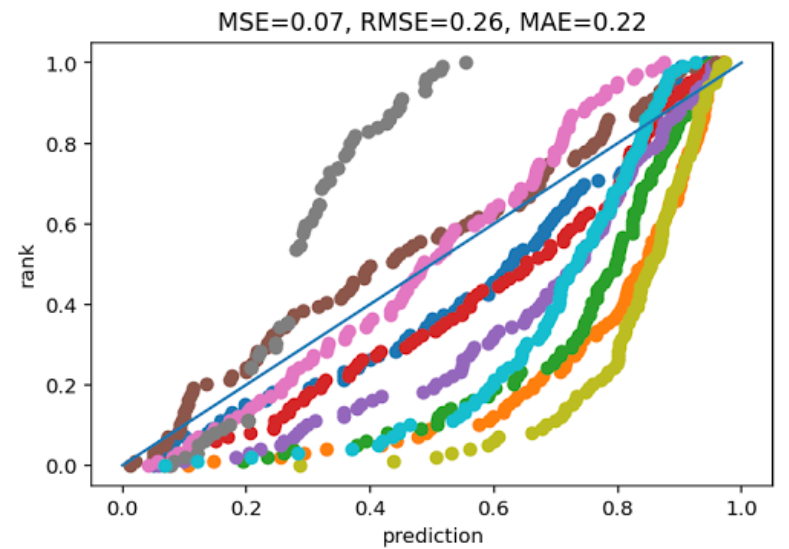
\includegraphics[width=0.45\columnwidth]{calibration_curve.png}}
    \end{subfigure}
    \begin{subfigure}{
    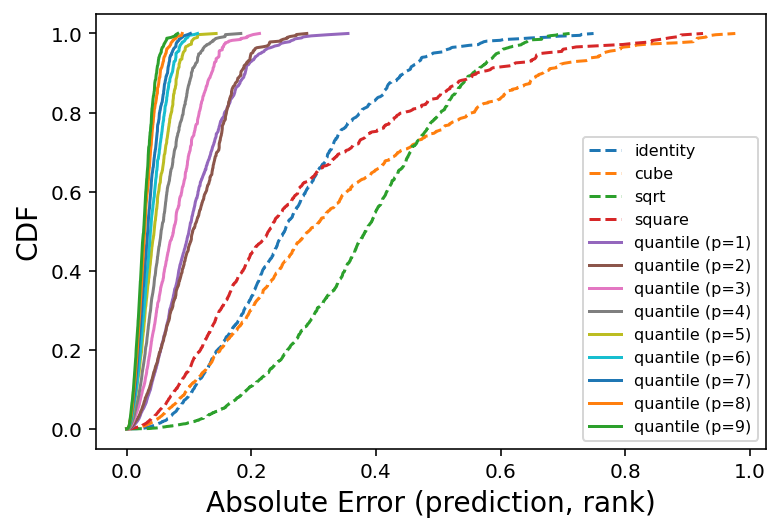
\includegraphics[height=115px]{error_rate.png}}
    \end{subfigure}
    \vspace{-.1in}
    \caption{Results on reward models trained on the Anthropic helpfulness preference dataset. (left) Scatter plot of reward scores and best-of-n ranks on a random sample of 10 prompts in the Anthropic helpfulness dataset. Note that the model shows miscalibration on most prompts, with the degree of miscalibration varying by prompt.
    %
    (right) Plot of CDF of absolute error (AE). Observe that per-prompt quantile based methods have low AE with high probability, where as prompt-agnostic transformations have high AE typically. \theertha{ananth: for the right plot, should it be just absolute error? what is the mean take over?}
    %
    }
    \label{fig:1}
    \vspace{-.1in}
\end{figure}

\subsection{Calibrated rewards improve standard win rate}
As a sanity check of \iapo, we first measure the performance when there is no inference-time procedure applied. Without any inference-time procedure, the optimization objective is \textit{standard win rate}, and we compare the performance of \ctrl\ (using an identity transform) against other relevant reward optimization baselines that are known to be (almost) win rate optimal, such as IPO \citep{azar2023general} and Best-of-N distillation \citep{gui2024bonbonalignmentlargelanguage, amini2024variationalbestofnalignment, sessa2024bondaligningllmsbestofn}. Specifically, we calibrated the reward model for helpfulness and harmlessness %
of the base model fine-tuned on preferred responses using Algorithm~\ref{alg1} with $p=1$. %
In Figure \ref{fig:winrate}, we find that compared to IPO and BoNBoN, the calibrated reward optimization achieves better win rate-KL trade-offs. We attribute this gain to a more efficient computation of win rate on training data using $m$ samples from the base model, as opposed to relying of existing pairwise comparison data during KL-RL. Further, we find that the reward transformations applied on the calibrated reward perform similar to each other, thus validating the theoretical results of \cref{sec:ctrl}. We also find that reducing the calibration error with more anchors or by varying $m$, leads to better win rate vs KL tradeoffs (see  \cref{sec:more_anchors}).

\begin{figure}
    \centering
    \begin{subfigure}
    {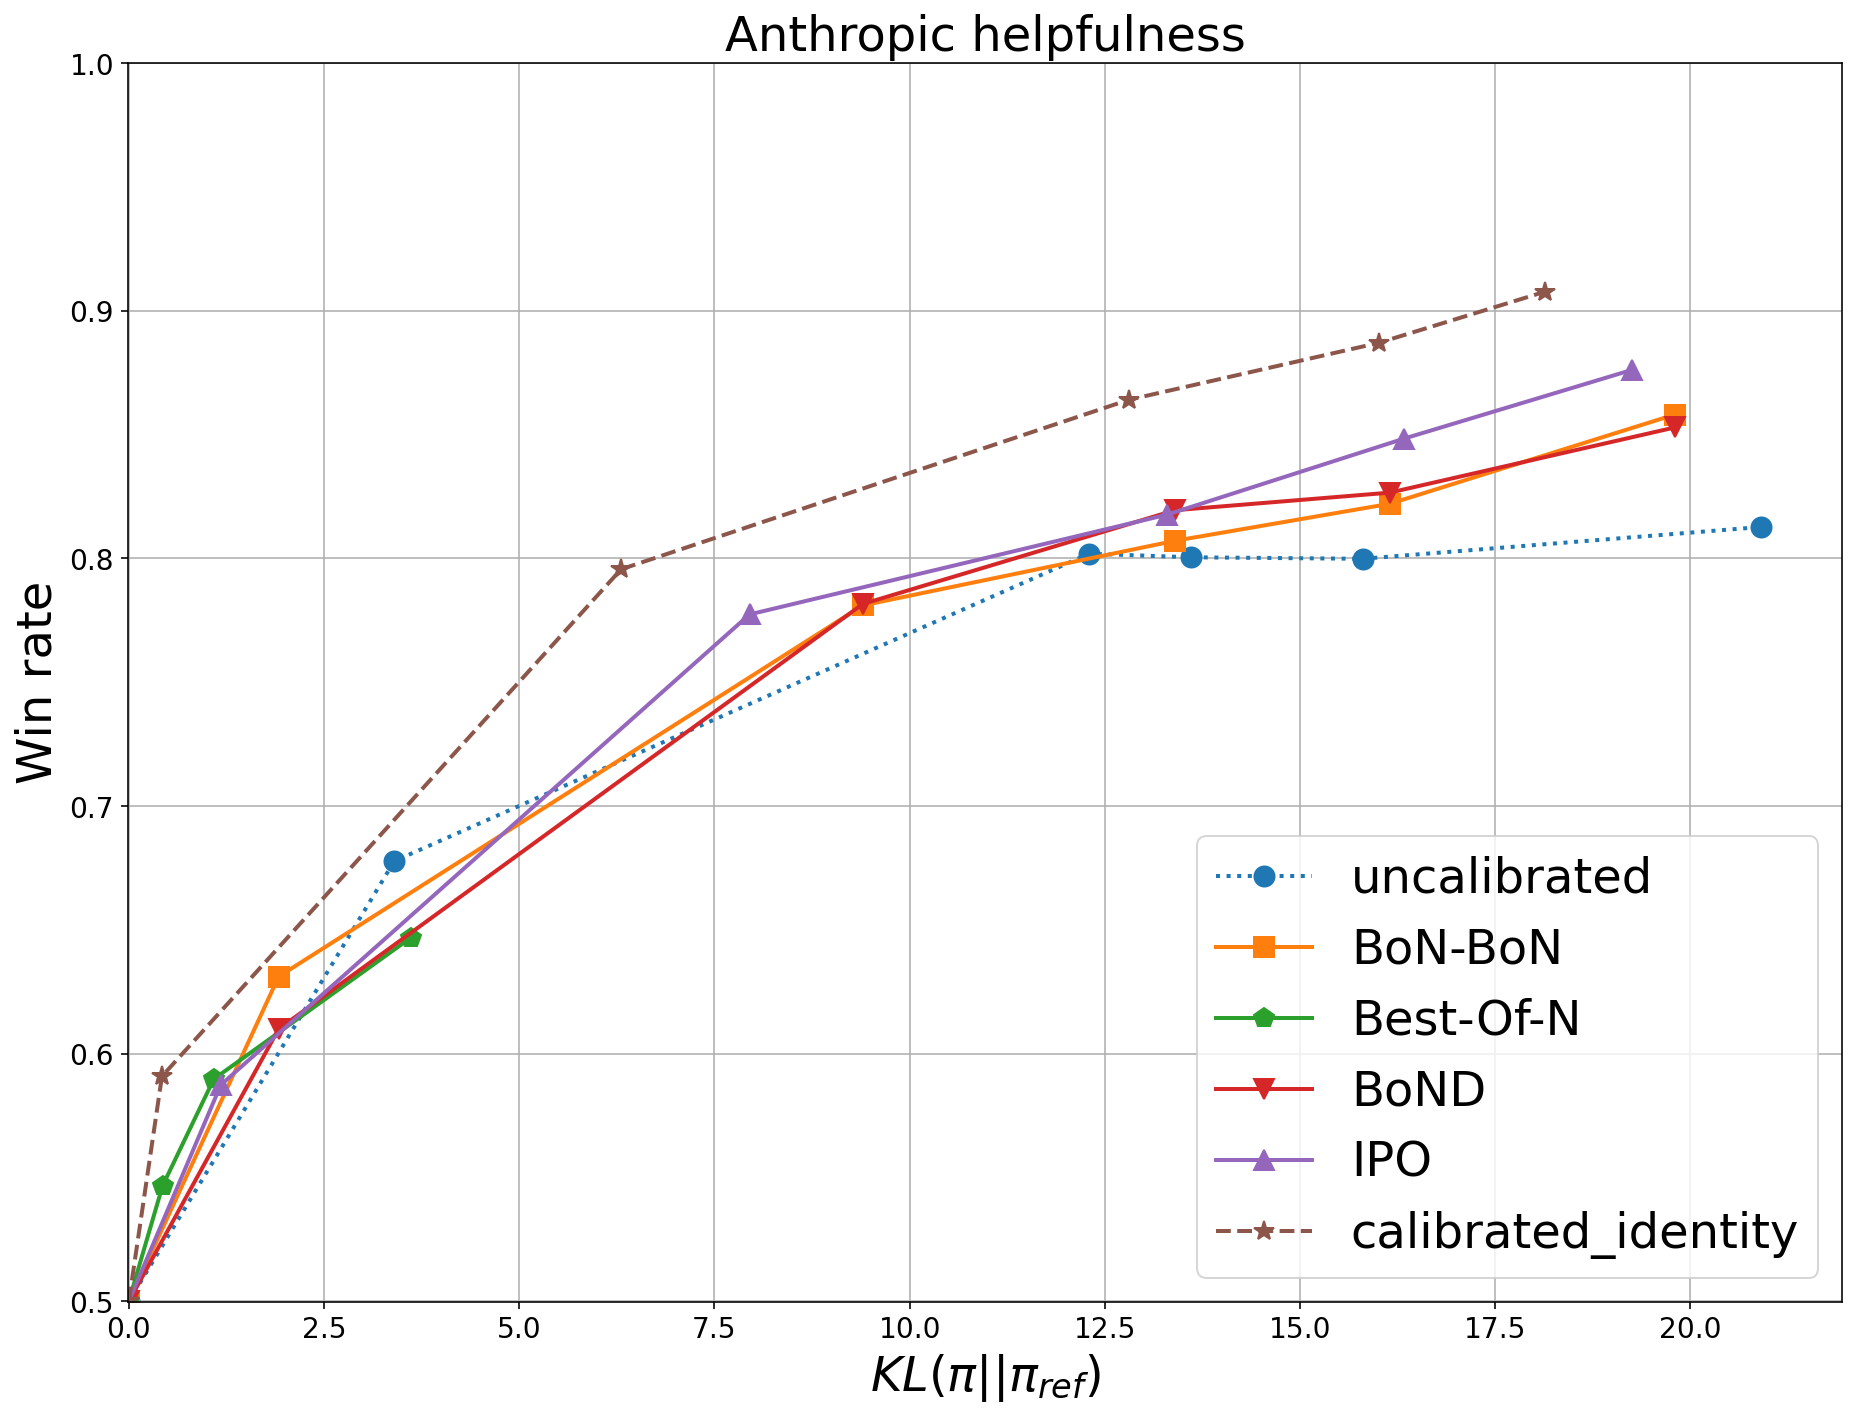
\includegraphics[width=0.45\columnwidth]{helpfulness_winrate.png}}
    \end{subfigure}
    \begin{subfigure}{
    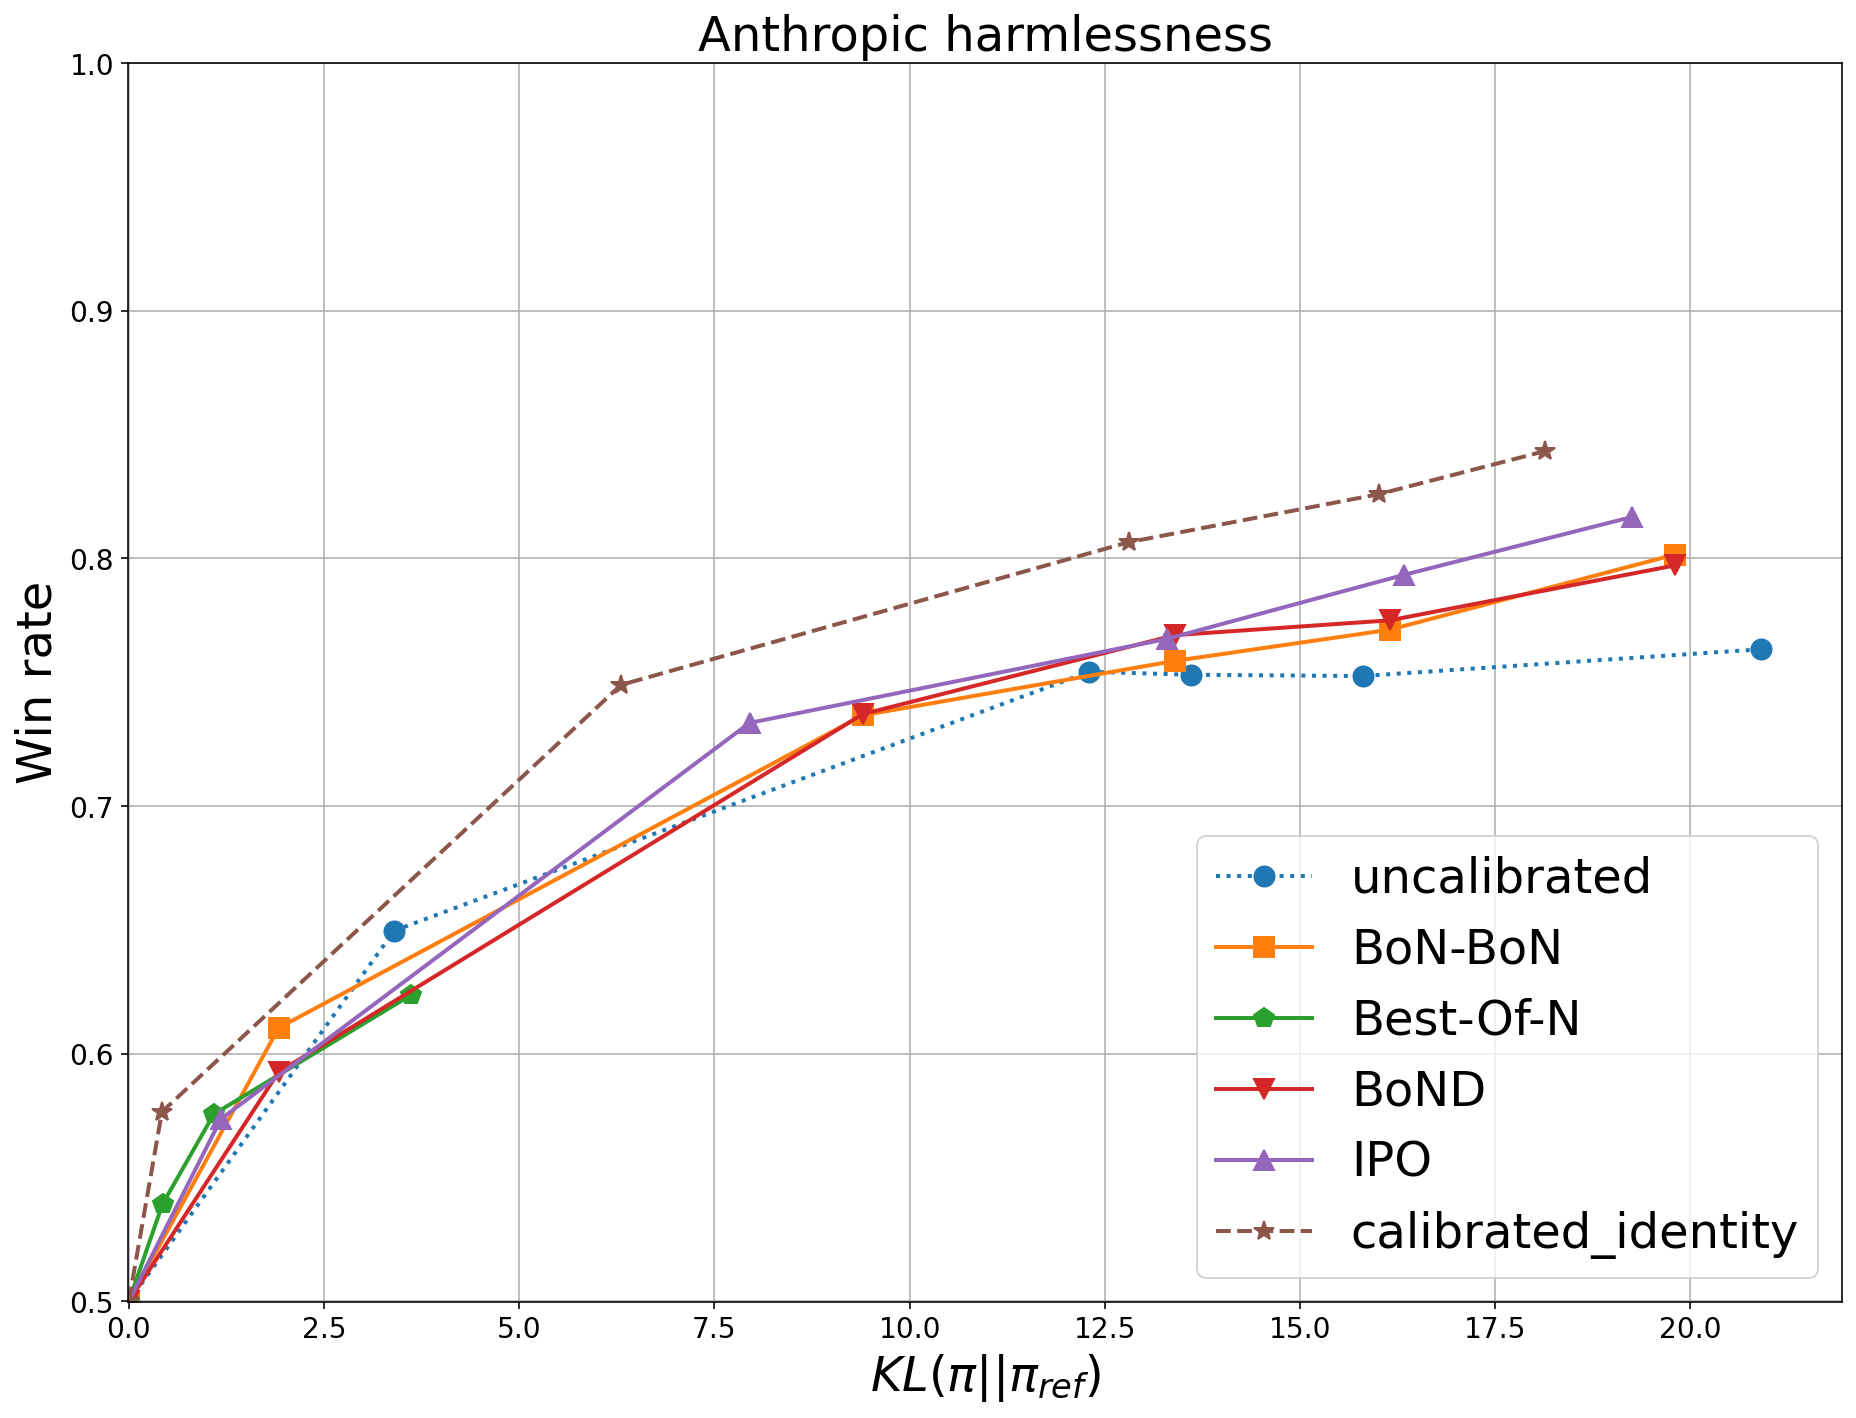
\includegraphics[width=0.45\columnwidth]{win_rate_harmlessness.png}}
    \end{subfigure}
    \caption{Calibrating the helpfulness and harmlessness reward improves average win rate (identity transformation).} 
    %
    \label{fig:winrate}
\end{figure}

%
%
\subsection{\ctrl\ improves \bofn}
%
For the helpfulness objective in the Anthropic dialog dataset, we aim to optimize the Best-of-$N$ performance of the aligned model through the exponential transformation of the calibrated rewards. We measure the win rate against the Best-of-$N$ of the base policy model ($N$=4). In Figure \ref{fig:2} we see that calibration based on the median rewards per-prompt achieves $8-12\%$ higher Best-of-$N$ win rates as compared to the uncalibrated model on helpfulness objective. The  exponential transformation of the calibrated reward outperforms the rest of the models. We find that the exponential factor of $t=10$ works best as simulated by our framework on a toy-setting (see Section~\ref{sec:ctrl}). Further, we show that these gains hold for varying values of $N (2, 32)$ (see Appendix~\ref{sec:more_compute}).

\subsection{\ctrl\ improves \wofn (\bofn jailbreaks)}
For the harmlessness objective in the Anthropic dialog dataset, we aim to improve the Worst-of-n performance of the aligned policy model to improve safety against adversarial actors \citep{hughes2024bestofnjailbreaking}. Here, we use the negative exponential transformation $t<0$. In Figure~\ref{fig:2} we see that calibration based on the median rewards per-prompt achieves $4-9\%$ higher Worst-of-$N$ win rates as compared to the uncalibrated model. The negative transformation of the calibrated reward outperforms the rest of the models, with $t=-10$ performing the best: again identified as the optimal value per our simulation in a toy setting (see Section~\ref{sec:ctrl}).
%

\begin{figure}
    \centering
    \begin{subfigure}{
    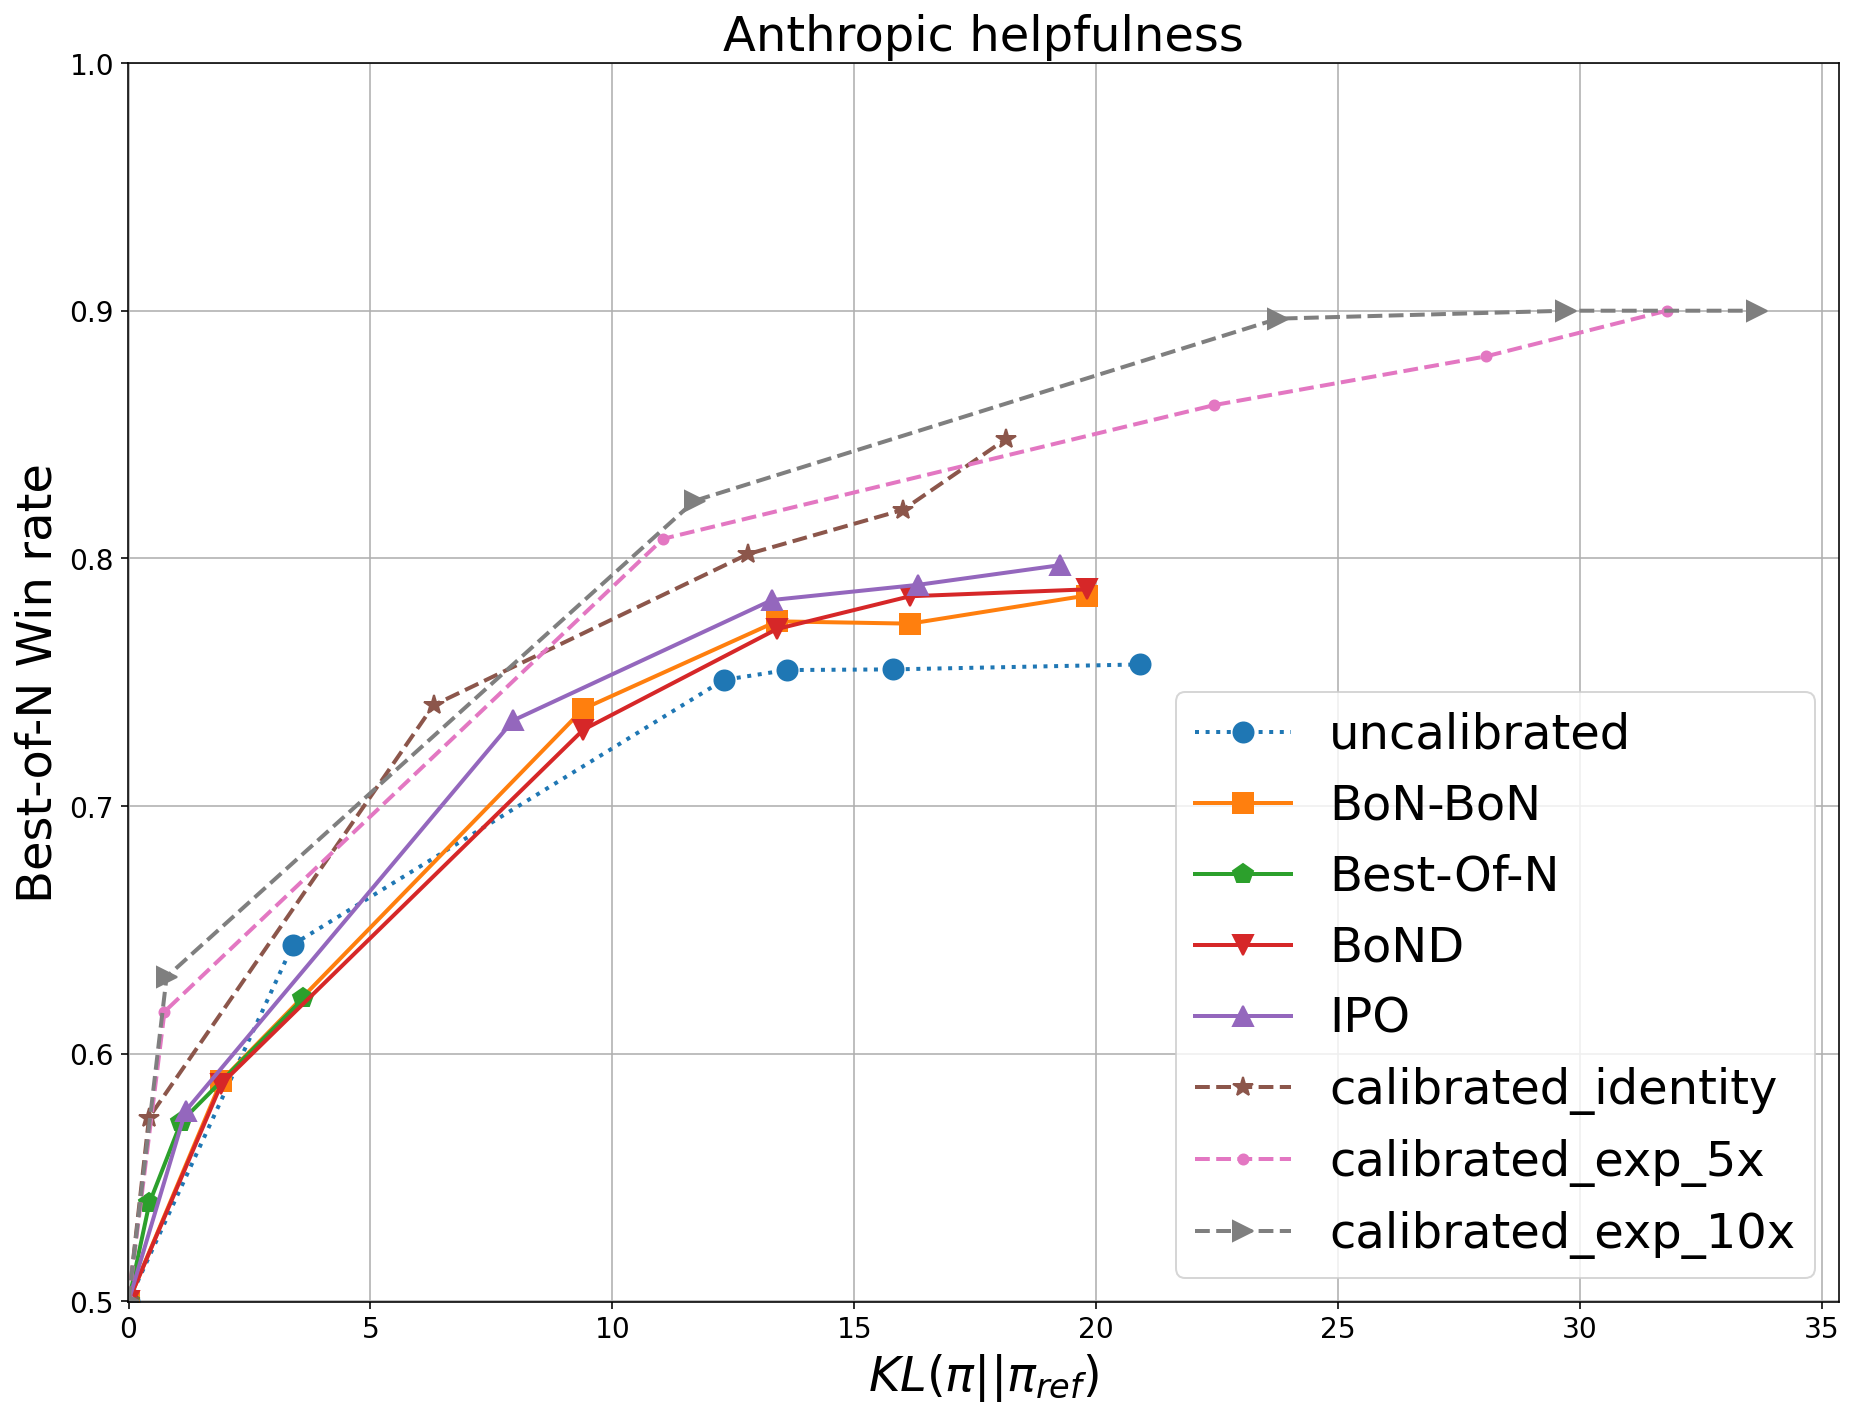
\includegraphics[width=0.45\columnwidth]{bobo-win_rate_helpfulness.png}}
    \end{subfigure}
    \begin{subfigure}{
    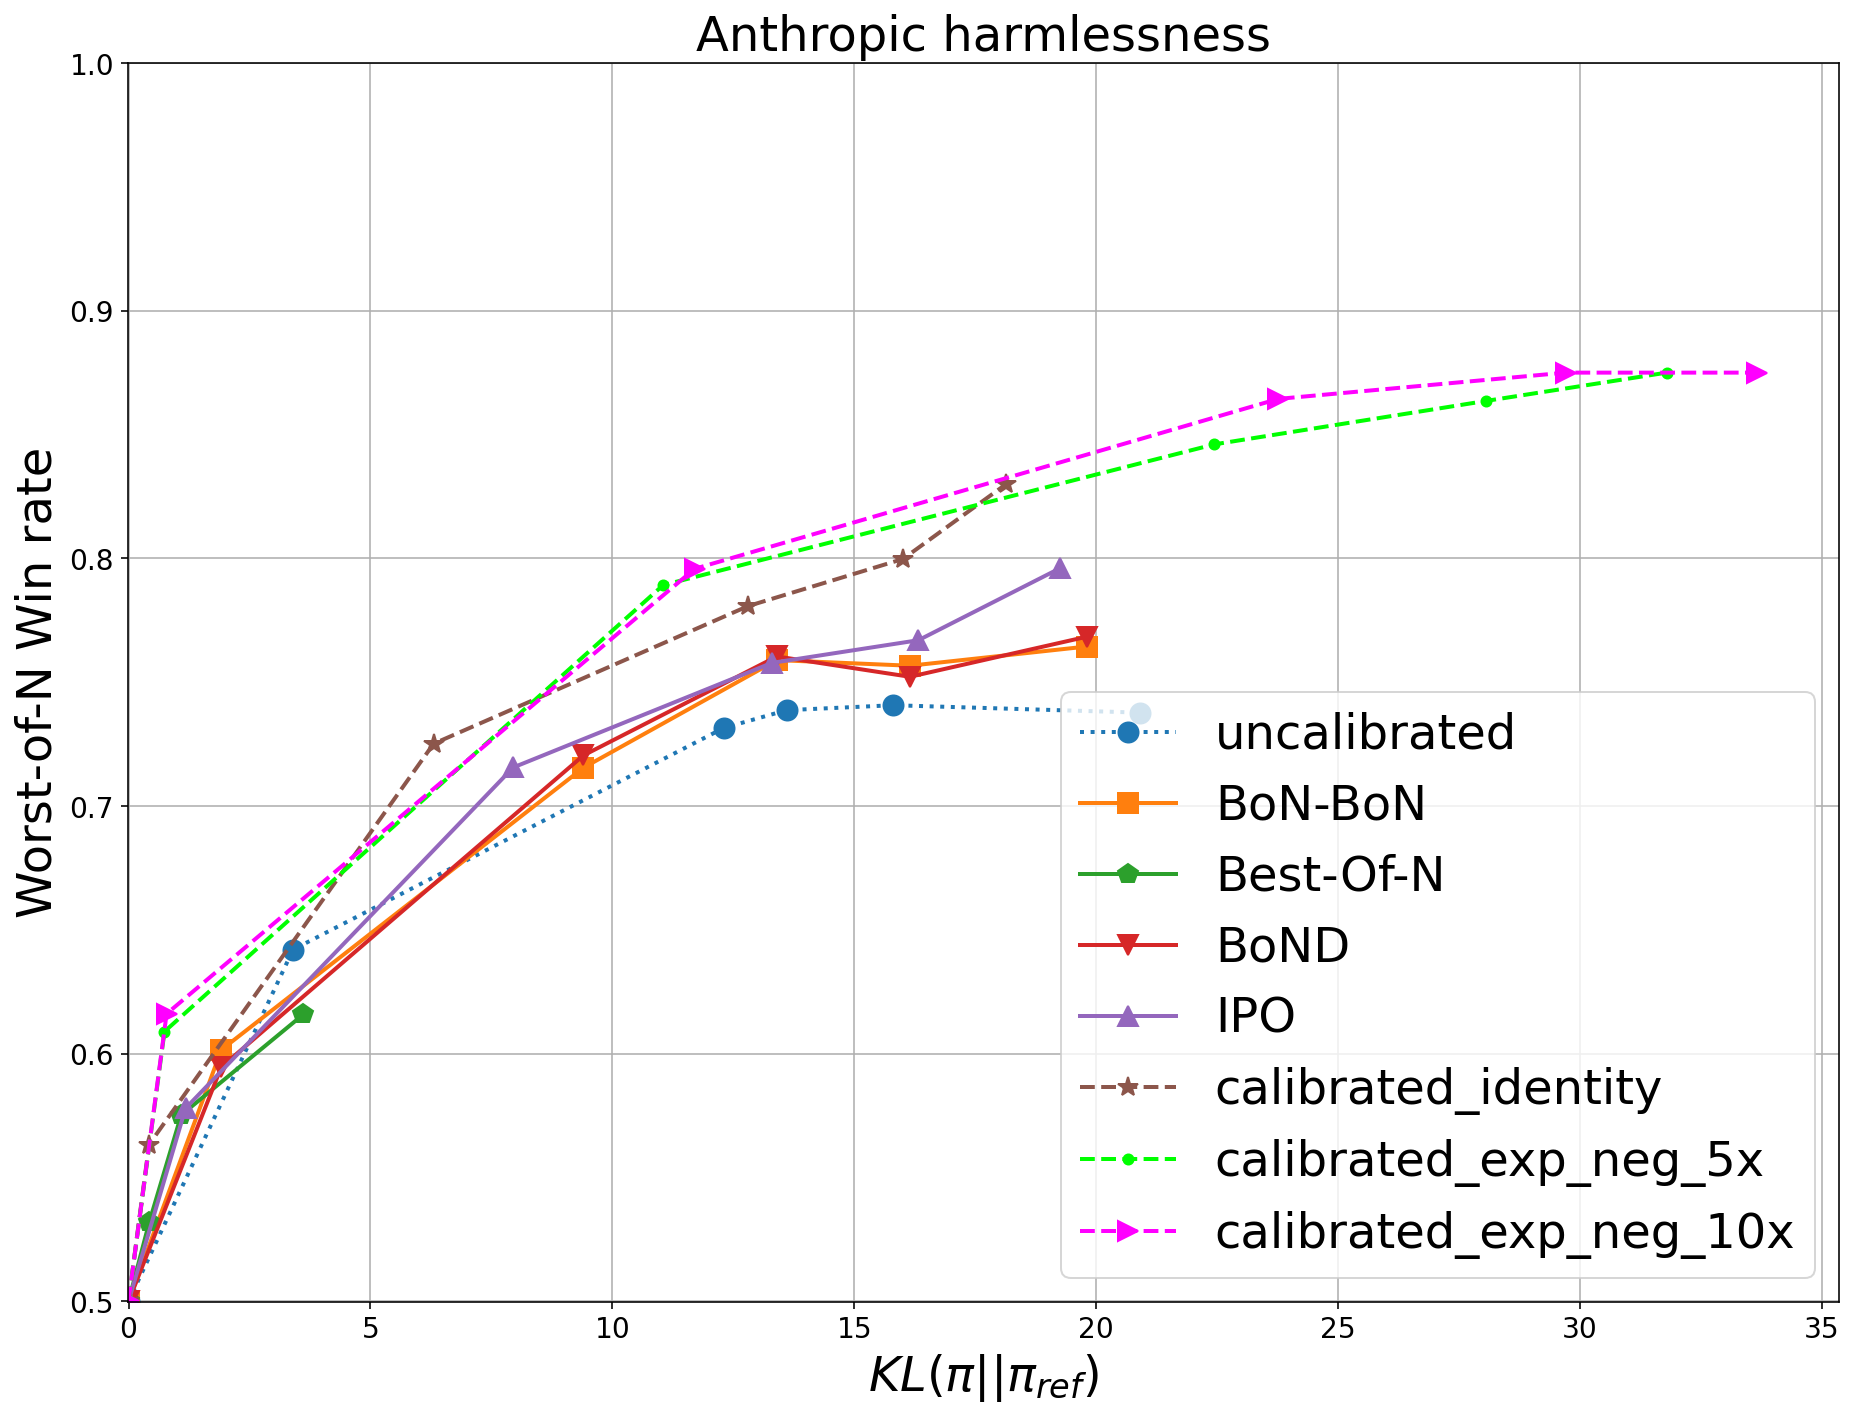
\includegraphics[width=0.45\columnwidth]{worst-of-n-harmlessness.png}}
    \end{subfigure}
    \caption{Calibration improves Best-of-$N$ and Worst-of-$N$ win rates for helpfulness (left) and harmlessness (right) objectives in the Anthropic dialog dataset respectively. We report win rate against the Best-of-$N$ and Worst-of-$N$ rewards of the base SFT model responses on the test split as measured by the PaLM-2 M reward model trained on the helpfulness and harmlessness data respectively.}
    \vspace{-.1in}
    \label{fig:2}
\end{figure}

%

%

%
%
%
%
%
%
%
%
%
%
%
%
%
%



%
%
%
%
%
%
%
%
%
%
%
%
%
%



%




%



\section{Related work} \label{sec:related}

%
%
%
%

\textbf{Inference-time compute.}
Test-time compute has been leveraged in recent work \citep{snell2024scaling, brown2024large, wu2024empirical} to achieve better win rate vs KL tradeoffs from the aligned models including controlled decoding \citep{mudgal2023controlled, chakraborty2024transfer}, 
Monte Carlo tree search \citep{chaffin-etal-2022-ppl, scialom2021beam, zhaoprobabilistic2024}, 
iterative jailbreak query refinement~\citep{pair}, and model-chaining within agentic frameworks~\citep{gurreal2024}. Best-of-N (\bofn) is also used as an evaluation metric in code and natural language generation benchmarks \citep{stiennon2020learning, chen2021evaluating}. Further, Worst-of-N (\wofn) is a popular jailbreaking strategy for adversarial actors to elicit unsafe text from large language models \citep{hughes2024bestofnjailbreaking}. Prior work has largely focused on approximating inference-time solutions during training time through sampling \citep{gui2024bonbonalignmentlargelanguage, amini2024variationalbestofnalignment}, distillation \citep{sessa2024bondaligningllmsbestofn}, and decoding \citep{qiu2024treebon}. Our work is orthogonal to this body of work as they assume that no inference-time procedure is applied, but rather attempt to approximate it during training. We show that our theoretical framework generalizes IPO~\citep{azar2023general} and best-of-$N$ distillation~\citep{gui2024bonbonalignmentlargelanguage, amini2024variationalbestofnalignment, sessa2024bondaligningllmsbestofn} as special cases. 

We are motivated by recent work that apply meta-generation procedures \citep{welleck2024decoding} at inference-time such as chaining prompted models \citep{brown2024large}, problem decomposition through chain-of-thought \citep{wei2022chain}, Best-of-N reranking \citep{collins-koo-2005-discriminative, charniak-johnson-2005-coarse, pauls-klein-2009-k} applied on reasoning traces \citep{o1}.  Our \iapo\ framework was also motivated by complex inference-time strategies that involve transformation techniques such as refinement \citep{madaan2024self}, majority voting \citep{wang2022self}, or using the generator as input to other search algorithms \citep{yao2024tree}, that have outperformed other models for harder tasks. In this spirit, our framework allows to get additional gains in aligning models with such inference-time procedures deployed in the future.

%


%
%

\textbf{Reward miscalibration.}
Reward miscalibration or hacking has been studied extensively in recent work \citep{amodei2016concrete, pang2022reward, gao2023scaling}. The hypotheses behind reward hacking can be broadly categorized into 3 themes: (1) reward underspecification, (2) training-serving skew between pairwise and pointwise reward models, (3) dominant reward due to adhoc transformations.
%
%
%
%
Reward models suffer from \textit{underspecification} due to under-specified training data \citep{skalse2022defining} by capturing spurious correlations in the data \citep{pan2022effects}. Methods to mitigate this often include training on non-overlapping splits during reward model fine-tuning \citep{bai2022training} and ensembling \citep{coste2023reward, eisenstein2023helping}. Our \ctrl\ method can be easily augmented with such data interventions in reward learning.

\textbf{KL-RL solvers.}
Training reward models on pairwise preference data, and then using it as pointwise scorers during reinforcement learning poses problems of transitive inconsistency. To mitigate this problem, optimization techniques that directly incorporate the pairwise preference data during offline reinforcement learning have been proposed \citep{rafailov2024direct, azar2023general}. Further, calibrating model probabilities to reflect rank-order generated sequences by quality metrics have been proposed \citep{zhao2022calibrating}. We share the motivation behind these methods, while additionally recognizing the need to calibrate the rewards against the base policy on which we are aligning.

When aligning language models for multiple objectives, aggregating the rewards via a weighted sum \citep{bai2022training, wu2024fine} is known to result in reward hacking of one of the dominant rewards. Thresholding the effect of individual rewards \citep{moskovitz2023confronting} or changing the weights of the training data \citep{bai2022training}, however requires costly hyper-parameter fine-tuning and retraining without the ability to reason about the hyperparameters and their effects on the reward-tradeoffs. Reward transformation techniques that calibrate against a reference reward is effective at mitigating domination of one reward \citep{wang2024transforming}, but implicitly assumes that the reward aggregation function is a logical "AND" of all rewards, heavily penalizing under-performance on any of the rewards. Motivated by the success of exponential tilting for focusing on high/low quantiles~\citep{li2023tilted}, we also show that \ctrl with exponential reward transformation achieves near-optimal inference-time win rate vs KL divergence tradeoffs, surpassing the performance of methods such as IPO~\citep{azar2023general} that target to optimize standard win rate vs KL divergence tradeoffs. In this paper, we show that calibration as a first-step can help ground reward transformations based on the final inference-time procedure applied. Further, we build on recent work that show the theoretical guarantees of Best-of-$N$ sampling \citep{beirami2024theoretical,gao2023scaling,mudgal2023controlled} over most reinforcement learning optimization techniques to ground our calibration and transformation method.




%
%
%
\vspace{-.1in}
\section{Concluding Remarks} 
\label{sec:conclusion}
\vspace{-.1in}
In this paper, we have shown that existing win rate optimal alignment procedures are sub-optimal when inference-time procedures are applied on aligned language models. As models equipped with inference-time procedures such as reasoning, best-of-$N$, majority voting continue to outperform models which do not use such procedures, we study the question of how to learn inference-aware optimally aligned language models. While learning optimal solutions for general inference-time procedures is intractable, we propose \iapo\ --- a framework that optimizes for inference-time win rate, and provide theoretical guarantees of finding an optimal inference-aware aligned model. Our framework generalizes prior work on win rate optimal solutions \citep{azar2023general, gui2024bonbonalignmentlargelanguage}. We further show that, for any inference time procedure, such an optimal model can be learned through KL-RL optimization using reward transformation. For a class of transformations that rely only on the rank of rewards, calibration of said rewards into a uniform distribution allows us to search efficiently for the optimal reward transformation through empirical simulation. 

We demonstrate the efficacy of this framework, by transferring findings from empirical simulation to real-world tasks and propose \ctrl\ --- a calibrate-and-transform reinforcement learning solver for ranking based inference-time procedures --- and particularize it to Best-of-$N$ sampling (\bofn) and jailbreaking (\wofn). Empirically, we demonstrate on Anthropic dialog helpfulness and harmlessness datasets that, (1) in the standard setting when no inference-time procedure is applied, \ctrl with identity reward transformation achieves competitive or slightly better performance compared to a variety of SOTA methods for optimizing standard win rate (2) when inference-time procedures are applied, we outperform inference-time win rate vs KL tradeoffs compared to existing preference optimization methods by 8-12\% for \bofn and 4-9\% for \wofn inference-time procedures respectively. 

Future work includes finding efficient solvers for complex inference-time procedures based on \iapo that do not rely on the rank of rewards assigned to samples from the base policy model, e.g., reasoning \citep{o1,xie2024calibrating}. Further, practical solvers for reward aggregation of multiple competing objectives at inference-time could also be explored. From a theoretical standpoint, the generalizability of our inference-aware alignment approach to upstream tasks such as supervised fine-tuning or pre-training needs to be studied.

%
%


\bibliography{main}
\bibliographystyle{iclr2025_conference}
%
\clearpage
\appendix
%

\section{Missing proofs}\label{app:proofs}
\subsection{Proof of \cref{thm:exisitence_informal}}
We start by stating the policy obtained by KL-regularized RL problem,  which can be obtained by standard arguments in the literature (\eg, \citep{korbak2022rl, rafailov2024direct, yang2024asymptotics}).

\begin{lemma}\label{lem:kl_rl}
The solution to the optimization problem in  \cref{def:kl_rl} satisfies
\[
    \pi_{r, \reg}^*(\by \mid \bx) \propto \bp(\by \mid \bx) \exp\Paren{\frac{r(\bx, \by)}{\reg}}.
\]
\end{lemma}

\begin{proof}[Proof of \cref{thm:exisitence_informal}]
Let $\pi_T^*$ be a solution to the optimization problem in \cref{eqn:kl-constrained-ppwr}. Note that for all $\by$ such that $\pi_T^*(\by \mid \bx) > 0$, we must have $\bp(\by \mid \bx) >0$ since otherwise the KL divergence would become infinite.

Then setting
%
$$\tr(\bx, \by)  =  \reg \log(\pi_T^*(\by \mid \bx) / \bp(\by \mid \bx))$$ in \cref{eqn:kl-rl-tr} leads to the solution $\pi_T^*$ being its optimal solution as shown in \cref{lem:kl_rl}.
\end{proof}


\subsection{Proof of \cref{lem:coupled}}
We first prove the following auxiliary lemma that we need in the proof.
\begin{lemma}\label{lem:pp_win_rate_decompose}
For any inference-time procedure $\pp$, we have
\[
    W^\pp_r(\pi_1 \succ \pi_2 \mid \bx) = \sum_{\bz} \qt_{r, T(\pi_2)}(\bx, \bz) T(\pi_1)(\bz \mid\bx).
\]
\end{lemma}
\begin{proof}
The proof follows from the following identities:
    \begin{align*}
     W^\pp_r(\pi_1 \succ \pi_2 \mid \bx)&  = \E_{\bz \sim \pp(\pi_1)(\cdot \mid \bx), \by \sim \pp(\pi_2)(\cdot \mid \bx)} \left\{w_r(\bz, \by \mid \bx)\right\} \\
     & = \E_{\bz \sim \pp(\pi_1)(\cdot \mid \bx)} \left\{\E_{\by \sim \pp(\pi_2)(\cdot \mid \bx)}\left\{w_r(\bz, \by \mid \bx)\right\} \right\} \\
     & =  \E_{\bz \sim \pp(\pi_1)(\cdot \mid \bx)} \left\{ \qt_{r, T(\pi_2)}(\bx, \bz) \right\} \\
     & = \sum_{\bz} \qt_{r, T(\pi_2)}(\bx, \bz) T(\pi_1)(\bz \mid\bx).
    \end{align*}
\end{proof}

\begin{proof}[Proof of \cref{lem:coupled}]
Note that \cref{eqn:kl-constrained-ppwr} has an implicit constraint that $\pi(\cdot \mid \bx)$ must be a valid distribution, \ie
\[
\sum_{\by} \pi(\by \mid \bx) = 1.
\]

Hence adding the Lagrangian multiplier, we get the following Lagrangian form
\[
    \cL(\pi(\cdot \mid \bx), \alpha) = W^\pp_r(\op \succ \bp \mid \bx) -\reg \KL(\op(\cdot \mid \bx) \| \bp(\cdot | \bx)) + \alpha \Paren{\sum_{\by} \pi(\by \mid \bx) - 1}.
\]

By method of Lagrange multipliers, we have that the solution to \cref{eqn:kl-constrained-ppwr} must be a stationary point of $\cL(\pi(\cdot \mid \bx), \alpha)$. And hence
\[
\mathbf{0} = \frac{\partial \cL(\pi(\cdot \mid \bx), \alpha)}{\partial   \pi(\by\mid\bx)} = \frac{\partial W^\pp_r(\op \succ \bp \mid \bx)}{\partial   \pi(\by\mid\bx)} - \beta\Paren{\log\frac{\op(\by \mid \bx)}{\bp(\by \mid \bx)} + 1} + \alpha.
\]

Setting 
\[
    \tr(\bx, \by) = \frac{\partial W^\pp_r(\op \succ \bp \mid \bx)}{\partial   \pi(\by\mid\bx)},
\]
we get 
\[
\log\frac{\op(\by \mid \bx)}{\bp(\by \mid \bx)}  = \frac{ \tr(\bx, \by) + \alpha }{\beta} - 1.
\]
And hence
\[
    \op(\by \mid \bx) \propto \bp(\by \mid \bx) \exp\Paren{\frac{\tr(\bx, \by)}{\beta}}.
\]

It remains to prove \cref{eqn:reward_expand}. 
Plugging in $\pi_1 = \pi$, $\pi_2 = \bp$ to \cref{lem:pp_win_rate_decompose}, and taking partial derivative with respect to $\pi(\by \mid \bx)$ on the right hand side completes the proof.
\end{proof}

\subsection{Proof of \cref{lem:monotone}}
If $r(\bx, \by) \ge r(\bx, \bz)$, we have $\forall \by'$,
\[
w_r(\by, \by' \mid \bx) \ge w_r(\bz, \by' \mid \bx).
\]

Hence 
\begin{align*}
    \qt_{r, \bp}(\bx, \by) =  \mathbb{E}_{\by' \sim \pi(\cdot \mid \bx)} w_r(\by, \by' \mid \bx) \ge  \mathbb{E}_{\by' \sim \pi(\cdot \mid \bx)} w_r(\bz, \by' \mid \bx) = \qt_{r, \bp}(\bx, \bz). 
\end{align*}


\subsection{Proof of \cref{lem:canonical}}
The proof follows from the fact that for all $\bx$ and $\by$
\begin{align}
      \car_{g(r), \bp} (\bx, \by) &= 
    \E_{\bz \sim \bp} \left\{ \mathbf{1}[g(r(\bx,\by)) > g(r(\bx,\bz))] + \frac{1}{2}  \mathbf{1}[g(r(\bx,\by)) = g(r(\bx,\bz))]\right\} \nonumber \\
    & =\E_{\bz \sim \bp} \left\{ \mathbf{1}[r(\bx,\by) > r(\bx,\bz)] + \frac{1}{2}  \mathbf{1}[r(\bx,\by) = r(\bx,\bz)]\right\} \label{eq:step-monotone}\\
      & = \car_{r, \bp} (\bx, \by), \nonumber
\end{align}
where~\eqref{eq:step-monotone} follows from monotone increasing property of $g.$

\subsection{Proof of \cref{lem:reward_uniform}}

To show that $\car_{r, \bp}(\bx, \by) \sim {\rm Unif}([0, 1]),$ it would be enough to show $\forall u \in [0, 1]$,
\[
    \text{Pr}_{\by \sim \bp}\Paren{\car_{r, \bp}(\bx, \by) \le u} = u. 
\]
\begin{align*}
     \text{Pr}_{\by \sim \bp}\Paren{\car_{r, \bp}(\bx, \by) \le u} & =  \text{Pr}_{\by \sim \bp}{r(\bx, \by) \le r(\bx, \by_{u, \bx})}  \\
     & = \car_{r, \bp}(\bx, \by_{u, \bx}) \\
     & = u,
\end{align*}
completing the proof.


\subsection{Proof of \cref{thm:calibrated_procedure}}

In this section, we will prove an extended version of \cref{thm:calibrated_procedure} below.

\begin{theorem}[Extended version of \cref{thm:calibrated_procedure}] \label{thm:calibrated_procedure_extended}
If $T$ is a calibrated inference-time procedure with mapping function $\calp$, for any continuous language model $\pi$, $\reg > 0$ and reward transformation function $\Phi$,  we have that 
\[W^T_r(\op^*_{\cR_{\Phi}, \reg} \succ \bp \mid \bx) = \frac{\int_{0}^1 \exp \Paren{\Phi(u)/\reg}g_T( F_{\Phi, \reg}(u) )\int_{0}^{u} g_T (u') \dd u' \dd u}{\int_{0}^1 \exp \Paren{\Phi(u)/\reg} g_T( F_{\Phi, \reg}(u) ) \dd u \int_{0}^1 \calp(u)\dd u} 
\] where $F_{\Phi, \reg}(u)= \frac{\int_{0}^u e^{\Phi(u')/\reg} \dd u'}{\int_{0}^1 e^{\Phi(u')/\reg} \dd u'}$, and \[\KL(\op^*_{\cR_{\Phi}, \reg} \| \bp) = 
\frac{1}{\reg}  \frac{ \int_{0}^1 \Phi(u) e^{\Phi(u)/\reg} \dd u }{\int_{0}^1 e^{\Phi(u)/\reg} \dd u} - \log \Paren{\int_{0}^1 e^{\Phi(u)/\reg} \dd u}.
\] 
And hence they are independent of $r$ and $\bp$.
\end{theorem}
\begin{proof}

In the proof, we consider the two language models $\op^*_{\cR_{\Phi}, \reg}$ and $\bp$ in the space of calibrated reward against the base policy $\bp$.  For any policy $\pi$, let $\qt_{r, \bp} \circ \pi(\cdot \mid \bx)$ be a distribution over $[0, 1]$ that outputs the calibrated reward $\qt_{r, \bp}(\bx, \by)$ of the sample $\by$ sampled from $\pi(\cdot \mid \bx)$. Then by \cref{lem:reward_uniform},
\[
    \qt_{r, \bp} \circ \pi(\cdot \mid \bx) \sim {\rm Unif}([0, 1]) .
\]

Similarly, using \cref{lem:kl_rl}, it can be shown that $\qt_{r, \bp} \circ \op^*_{\cR_{\Phi}, \reg}$ follows the distribution with density $\forall u \in [0, 1]$,
\[
    \qt_{r, \bp} \circ \op^*_{\cR_{\Phi}, \reg} (u) = \frac{ e^{\Phi(u)/\reg} }{\int_{0}^1 e^{\Phi(u')/\reg} \dd u'}.
\]

Note that since $r$ assigns distinct rewards to different $\by$'s and $\qt_{r, \bp}$ is a monotone transformation of $r$, we
have that

\begin{align*}
   \KL(\op^*_{\cR_{\Phi}, \reg} \| \bp) & =\KL( \qt_{r, \bp} \circ \op^*_{\cR_{\Phi}, \reg} \| \qt_{r, \bp} \circ \pi ) \\
   & = \int_{u = 0}^1 \frac{ e^{\Phi(u)/\reg} }{\int_{0}^1 e^{\Phi(u')/\reg} \dd u'} \log \frac{ e^{\Phi(u)/\reg} }{\int_{0}^1 e^{\Phi(u')/\reg} \dd u'} \dd u \\
   & = \frac{1}{\reg}  \frac{ \int_{u = 0}^1 \Phi(u) e^{\Phi(u)/\reg} \dd u }{\int_{0}^1 e^{\Phi(u)/\reg} \dd u} - \log \Paren{\int_{0}^1 e^{\Phi(u)/\reg} \dd u}.
\end{align*}

After the inference-time procedure $T$ is applied, we have that inference-time base policy satisfies
\[
    \qt_{r, \bp} \circ T( \bp) (u) = \frac{ g_T( u )}{\int_{0}^1 g_T( u' ) \dd u' }.
\]

For the inference-time aligned policy, we have that:
\[
    \text{Pr}_{\by \sim \op^*_{\cR_{\Phi}, \reg}(\cdot \mid \bx)}  \Paren{\qt_{r, \bp}(\bx, \by) \le u} = \frac{\int_{0}^u e^{\Phi(u')/\reg} \dd u'}{\int_{0}^1 e^{\Phi(u')/\reg} \dd u'},
\]
which is defined as $F_{\Phi, \reg}(u)$. And hence we have
\[
     \qt_{r, \bp} \circ T( \op^*_{\cR_{\Phi}, \reg}) (u) = \frac{ \exp \Paren{\Phi(u)/\reg}g_T( F_{\Phi, \reg}(u) )}{\int_{0}^1 \exp \Paren{\Phi(u)/\reg} g_T( F_{\Phi, \reg}(u) ) \dd u }.
\]
Thus, the inference-time win rate satisfies\footnote{Below we add an additional $\frac{1}{2}\idc{r(\bx, \by) = r(\bx, \bz)}$ to the win r.v for simplicity, which won't affect the result for continuous LMs.}
\begin{align*}
     W^T_r(\op^*_{\cR_{\Phi}, \reg} \succ \bp \mid \bx) 
    & = \E_{\by \sim \pp(\op^*_{\cR_{\Phi}, \reg})(\cdot \mid \bx), \bz \sim \pp(\bp)(\cdot \mid \bx)} \left\{\idc{r(\bx, \by) \ge r(\bx, \bz)} \right\}\\
    & = \E_{\by \sim \pp(\op^*_{\cR_{\Phi}, \reg})(\cdot \mid \bx), \bz \sim \pp(\bp)(\cdot \mid \bx)} \left\{\idc{\qt_{r, \bp}(\bx, \by) \ge \qt_{r, \bp}(\bx, \bz)} \right\}\\
    & = \text{Pr}_{u \sim  \qt_{r, \bp} \circ T( \op^*_{\cR_{\Phi}, \reg}), u' \sim  \qt_{r, \bp} \circ T( \bp)} \Paren{ u' \le u} \\
    & = \frac{\int_{0}^1 \exp \Paren{\Phi(u)/\reg}g_T( F_{\Phi, \reg}(u) )\int_{0}^{u} g_T (u') \dd u' \dd u}{\int_{0}^1 \exp \Paren{\Phi(u)/\reg}g_T( F_{\Phi, \reg}(u) ) \dd u \int_{0}^1 \calp(u)\dd u},
\end{align*}
completing the proof.
\end{proof}
%
%
%
%
%

%
%
%


\subsection{Proof of \cref{thm:wr_kl_bon_won}}
The KL divergence is the same as the KL divergence in \cref{thm:calibrated_procedure_extended}. The win rate can be obtained by plugging $g_{\bofn}(u) = u^{N-1}$ and $g_{\wofn}(u) = (1 - u)^{N-1}$ (as shown in \cref{lem:bofn_wofn}) into \cref{thm:calibrated_procedure_extended}.

%
\subsection{Proof of \cref{cor:coupled_won}}
We will show that \cref{cor:coupled_won} is a special case of \cref{lem:coupled} with a simple continuous language model. And by \cref{thm:calibrated_procedure}, we have the $\Phi$ can be generalized to arbitrary continuous language models.

Let $\bcY = [0,1]$. We assume the LMs and reward models are context-independent. We use $u \in [0, 1]$ to denote $\by$ and set the reward model to be $r(u) = u$. The base policy is a simple uniform distribution over $[0, 1]$, $\bp = \text{Unif}([0, 1])$. Let $F_{\pi}(u)$ be the CDF of $\pi$, then we have that the \bofn win rate is
\[
    W^{\bofn}_r(\pi \succ \bp \mid \bx) = 1 - N \int_{0}^1 F_{\pi}(u)^N u^{N-1} \dd u,
    \]
and \wofn win rate is
    \[
    W^{\wofn}_r(\pi \succ \bp \mid \bx) =  N \int_{0}^1 \Paren{1 - F_{\pi}(u) }^N (1-u)^{N-1} \dd u.
    \]
Plugging these into \cref{lem:coupled}, we have for \bofn, 
\begin{align*}
    \tr(u) & = \frac{\partial W^{\bofn}_r(\pi \succ \bp \mid \bx)}{\partial \pi(u)} \\
    & =  - N \int_{0}^1  v^{N-1} \frac{\partial F_{\pi}(v)^N}{\partial \pi(u)}\dd v \\
     & = - N \int_{0}^1  v^{N-1} F_{\pi}(v)^{N-1}\frac{\partial F_{\pi}(v)}{\partial \pi(u)}\dd v \\
    & = -N^2 \int_0^1 F_{\pi}(v)^{N-1} \idc{v \ge u} v^{N-1} \dd v \\
    & = -N^2 \int_u^1 F_{\pi}(v)^{N-1} v^{N-1} \dd v.
\end{align*}

For \wofn, we have
\begin{align*}
    \tr(u) & = \frac{\partial W^{\wofn}_r(\pi \succ \bp \mid \bx)}{\partial \pi(u)} \\
    & =  N \int_{0}^1  (1 - v)^{N-1} \frac{\partial \Paren{1 - F_{\pi}(v)}^N}{\partial \pi(u)}\dd v \\
     & = - N^2 \int_{0}^1  (1-v)^{N-1} (1 - F_{\pi}(v))^{N-1}\frac{\partial F_{\pi}(v)}{\partial \pi(u)}\dd v \\
    & = -N^2 \int_0^1 (1-v)^{N-1} (1 - F_{\pi}(v))^{N-1} \idc{v \ge u}\dd v \\
    & = -N^2 \int_u^1 (1-v)^{N-1} (1 - F_{\pi}(v))^{N-1} \dd v.
\end{align*}

\clearpage

%

%
%
%
%
%
%
%
%
%
%
%
    
%
%
%
%
%
%
%
%
%
%
%
%

%

%
%

%

\clearpage
\section{The role of KL divergence in model alignment}
\label{app:role-KL}

One question that arises is the role of the KL divergence regularizer in \cref{eqn:kl-constrained-ppwr}. In this section, we argue that the regularizer essentially enables multi-tasking between the SFT task and the RL task. 

Let's consider a log-linear model such that 
\begin{equation}
    \pi_\theta(y|x) = e^{\theta^T g(x, y) - A(\theta; x)} ,
\end{equation}
where $g(x,y)$ is  a fixed encoding of $(x, y)$, and $A(\theta;x)$ is the partition function normalizing the distribution.

\paragraph{Supervised finetuning (SFT).}
Let $D_\sft(x, y) = \mu(x) \times p_\sft(y|x)$ be the SFT data distribution. 
Then, the SFT task is
\begin{equation}
    {\theta}^*_\sft = \arg\min_\theta \mathcal{L}_\sft(\theta) \quad \quad \text{where} \quad \quad \mathcal{L}_\sft(\theta) := E_{(x, y) \sim D_\sft} \{ A(\theta; x) - \theta^\top  g(x, y)\},
\end{equation}
We further call $\p = \pi_{\theta^*_\sft}$.
\begin{lemma}
The SFT solution satisfies
\begin{equation}
    E_{x\sim \mu} \{\nabla_\theta A(\theta^*_\sft)\} = E_{(x,y) \sim D_\sft} g(x,y).
\end{equation}
\vspace{-.3in}
\label{lem:sft}
\end{lemma}
\begin{proof}
    This is a known property of exponential families. The proof follows by noticing  $\nabla_\theta \mathcal{L}_\sft(\theta^*_\sft) = 0.$
\end{proof}

\paragraph{KL-regularized reward optimization (RO).} Let $r$ be a reward function that determines the reward for each $(x,y).$ Let $\mathcal{L}_\ro(\theta) :=  E_{x \sim \mu} E_{y \sim \pi_\theta} r(x, y)$. Then, 
\begin{equation}
    \theta^*_{\bilevel, \beta} = \arg\min_\theta  \mathcal{L}_{\bilevel, \beta}(\theta) \quad\quad \text{where} \quad\quad \mathcal{L}_\bilevel(\theta ) :=  \KL(\pi_\theta \| \p) + \frac{1}{\beta}\mathcal{L}_\ro(\theta),
\end{equation}
where $\KL(\pi_\theta \| \p) = E_{x \sim \mu} \KL(\pi_\theta(\cdot|x) \| \p(\cdot|x))$.

\paragraph{Multi-tasking SFT and RO.} Now consider the following tasks
\begin{equation}
    \theta^*_{\multitask, \beta} = \arg\min_\theta \mathcal{L}_{\multitask, \beta}(\theta) \quad \quad \text{where} \quad \quad \mathcal{L}_\multitask(\theta) := \mathcal{L}_\sft(\theta) + \frac{1}{\beta} \mathcal{L}_\ro(\theta) .
\end{equation}

\begin{theorem}
For all $\beta \in \mathbb{R},$   we have $\theta^*_{\bilevel, \beta} = \theta^*_{\multitask, \beta}.$
\label{prop:role-of-KL}
\end{theorem}
\begin{proof}
    Notice that
\begin{align}
    \mathcal{L}_{\bilevel,\beta}(\theta) &= \KL(\pi_\theta \| \p) + \frac{1}{\beta} \mathcal{L}_\ro(\theta) \\
    &= E_{x \sim \mu}  \{A(\theta; x) - A(\theta^*_\sft; x) - (\theta- \theta^*_\sft)^\top \nabla_\theta A(\theta^*_\sft; x) \}  +\frac{1}{\beta}\mathcal{L}_\ro(\theta) \label{eq:bregman}\\
    & = E_{x \sim \mu} \{A(\theta; x) - A(\theta^*_\sft; x)\} - (\theta - \theta^*_\sft)^\top E_{(x,y) \sim D_\sft} g(x,y) + \frac{1}{\beta} \mathcal{L}_\ro(\theta) \label{eq:lemma1}\\
    &= \mathcal{L}_{\multitask, \beta}(\theta) + \mathcal{L}_\sft(\theta^*_\sft), \label{eq:last_ineq}
\end{align}
where \cref{eq:bregman} follows by noticing that KL divergence is a Bregman divergence in this setup, \cref{eq:lemma1} follows from Lemma~\ref{lem:sft}, and \cref{eq:last_ineq} follows from the definition of $\mathcal{L}_\sft(\theta)$ applied to $\theta$ and $\theta^*_\sft$. Hence, the minimizers of the two objectives are the same given that $$\mathcal{L}_{\bilevel,\beta}(\theta) = \mathcal{L}_{\multitask, \beta}(\theta)+ C,$$
completing the proof.
\end{proof}

Thus, effectively this proves that the KL-RL objective enables multi-tasking between the SFT stage and the reward optimization RL objective.
One may wonder why we did not pose the KL divergence regularizer on the transformed distributions through $\KL(T(\op)(\cdot \mid \bx) \| T(\bp)(\cdot | \bx))$ instead. Consider the Best-of-$N$ jailbreaking for example. While the adversary may be using the model to generate $N$ responses and choose the least safe one for jailbreaking, the model should possess the core capabilities for other types of inference-time usage for other tasks that is different from that of jailbreaking  (e.g., through chain-of-thought). Therefore, changing the KL divergence regularizer does not capture the fact that the model should remain suitable for all other tasks, and not just for the one for which it is getting aligned.
We also note that if we used $\KL(T(\op)(\cdot \mid \bx) \| T(\bp)(\cdot | \bx))$ instead, the problem would actually simplify to the standard alignment problem through a simple change of variables.

\clearpage



%
%
%
%
%

%
%
%
%
%
%


\clearpage
\section{Zero-shot prompt}
We also evaluate the win rate using a prompted PaLM-XL model with the following instructions:

\noindent\fbox{%
    \parbox{\textwidth}{%
You are a helpful assistant, that ranks AI assistants' responses by the quality of their answers.
The AI assistants try to be helpful, sophisticated, emotionally aware, and humble-but-knowledgeable.
Below are a series of dialogues between various people and an AI assistant, and the assistant tries to reply to the dialogue.

I want you to rank the responses of assistants.
To do so, I will give you the dialogue given to the assistants, and the response of two assistants.
Please rank the assistants based on which response would be more helpful, sophisticated, emotionally aware, and humble-but-knowledgeable.
All inputs are python dictionaries.

Here is the prompt:
\{{
    "dialogue": \{dialogue\},
\}}

Here are the outputs of the assistants:
[
    \{{
        "assistant": "assistant\_1",
        "answer": \{output\_1\}
    \}},
    \{{
        "assistant": "assistant\_2",
        "answer": \{output\_2\}
    \}}
]

Respond 1 or 2 to indicate the better output. Please provide the ranking that the majority of humans would give.
    }%
}

%
%
%
%
%
%
%
%
%
%
%
%
%
%


\clearpage
\section{The effect of anchor points on calibration}
\label{sec:more_anchors}
In this section, we analyze the effect of using more anchor points on results. First, we present the full algorithm for more than one anchor point in \cref{app:algorithm}.


\begin{algorithm}[ht]
\caption{Offline Approximate Calibration with arbitrary anchor points} \label{app:algorithm}
\begin{algorithmic}[1]
\Require Base policy $\bp$, (uncalibrated) reward model $r$, training prompts $\bx \in \mathcal{X}$, number of quantiles $p$, number of samples per prompt $m$. 
%
%
\ForAll{$\bx \in \mathcal{X}$}
\State Roll out $m$ i.i.d. samples from $\bp$ per training prompt $\bx$: $\bz_{j},\, j \in \{1...m\}$. %
%
\ForAll{$\ell \in \{0...p-1\}$}
\State $q_\ell = \frac{\ell+1}{p+1}$ 
\State $r_{q_\ell}(\bx) \leftarrow \text{top}_{ q_\ell \cdot m}(r(\bx, \bz_{1}), \ldots r(\bx, \bz_{m}))$ \quad {\color{blue}{select $(q_\ell \cdot m)^{\text{th}}$ smallest element}}
\EndFor
\EndFor
\State Define the calibrated reward function $\widehat{\car}_{r, \bp}(\bx, \by): \mathcal{X} \times \mathcal{Y} \to [0, 1]$ as follows:
\begin{align*}
{\log \widehat{\car}_{r, \bp}(\bx, \by)} = \log \bigl( r(\bx, \by) \bigr)  \cdot   \frac{  {\log \bigl( \frac{q_a + q_{b}}{2}}\bigr) }{\log \bigl( \frac{r_{q_a}(\bx) + r_{q_{b}}(\bx)}{2}\bigr) } ,
\end{align*}
where $a$ is the smallest number in $[0, p-1)$ such that $r_{q_a}(\bx) \geq r(\bx,\by)$, otherwise $a=0$. Similarly,  $b$ is the largest number in $[0, p-1)$ such that $r_{q_b}(\bx) \leq r(\bx,\by)$, otherwise $b=p-1$.

%
%
%
%
%
%
%
%
%
%
%

%
%
%
%
%
%
%
%
%
%
 \State \textbf{Output:} Calibrated Reward Function: $\widehat{\car}_{r, \bp}$ that assigns a calibrated reward for all prompts in the training set.
\end{algorithmic}
\end{algorithm}


\subsection{Better calibration leads to better gains}
The effectiveness of calibration can be better understood when we approximate the calibration with fewer number of rollouts: $n$. When $n=1$, we take one other rollout from the base policy model and use that as a reference reward, similar to \cite{wang2024transforming}, and with $n=3,5,7$, we approximate the median with this limited sample, and do the reward calibration. In Fig \ref{fig:3}(a), we find that calibration using more number of samples improves the win rate, with $n=1$ providing no gains in the KL vs win rate tradeoff. Additionally, in Fig \ref{fig:3}(b), when we calibrate with more anchor points, we find that the KL vs win rate tradeoffs improves as compared to the median-based calibration. This is further supported by the fact that with more anchor points, the calibration error is significantly reduced as shown in Fig \ref{fig:1}(b). Hence, we find that as the calibration error is reduced, we achieve better KL vs win rate tradeoffs, thus able to better implicitly approximate the best-of-n model. 

%
%
%
%
%
%
%
%
%
%

%

\begin{figure}
    \centering
    \begin{subfigure}{
    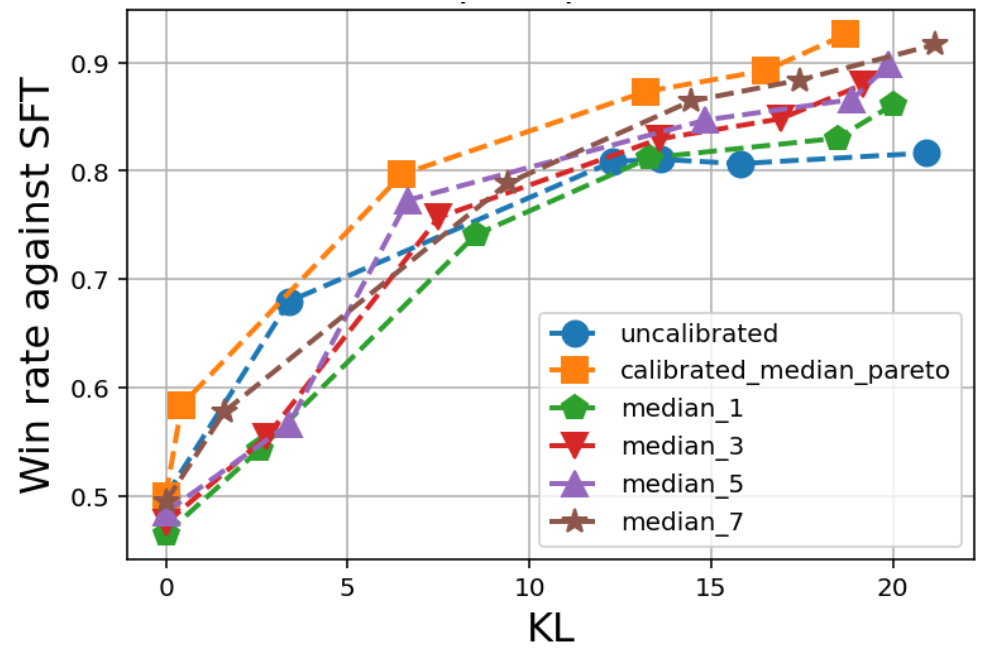
\includegraphics[width=0.45\columnwidth]{median_approximation.png}}
    \end{subfigure}
    \begin{subfigure}{
    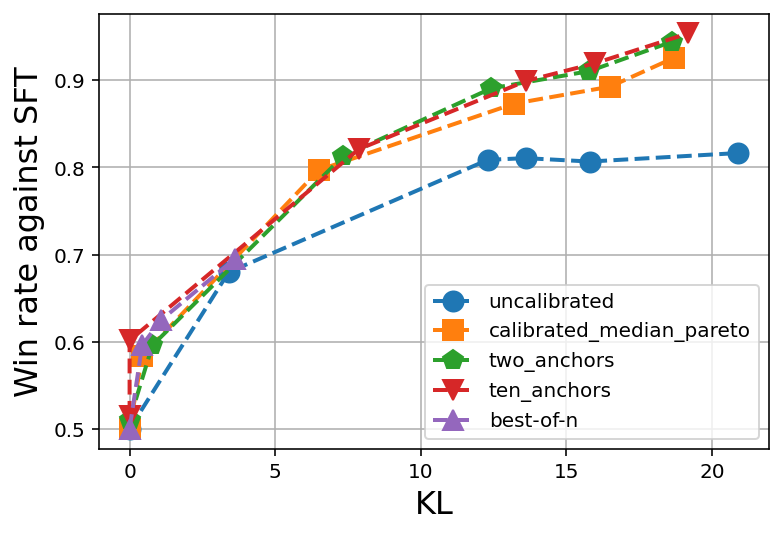
\includegraphics[width=0.45\columnwidth]{anchors_multiple.png}}
    \end{subfigure}
    \caption{(a) Calibration improves KL vs win rate tradeoff even when we approximate calibration of median approximated with n=7 samples, whereas with n=1,3,5, the gains in win rate for a fixed KL-budget is lower, but still outperforms the uncalibrated model at higher KL values. Using n=100 samples is (calibrate\_median\_pareto) provides the best tradeoff (b) Calibration with two or more anchor points per-prompt improves KL-winrate tradeoff, as compared to median-based approximation - however there is diminishing gains with ten anchor points as compared to using two anchor points.
    The win rate is measured using the PaLM-2 M reward model trained on the Anthropic helpfulness preference dataset.}
    \label{fig:3}
\end{figure}


\subsection{Calibration Reduces Reward Hacking}

We demonstrate that calibrated reward models are less susceptible to reward hacking, a phenomenon where models exploit spurious correlations in training data to optimize for reward signals instead of true task objectives.

To induce reward hacking, we injected specific phrases into the start of preferred responses of our preference datasets: ``Sorry, I can't help you with that'' for Harmlessness and ``Sure'' for Helpfulness. We then evaluated the model's accuracy on a poisoned evaluation set where these phrases were inverted (added to the \textit{unpreferred} responses). A significant drop in accuracy on this poisoned set would indicate reward hacking: a reliance on the spurious correlation.

Figure \ref{fig:reward_hacking} shows that calibrated reward models are far more robust to these manipulated correlations, maintaining higher accuracy compared to uncalibrated models. Note that the calibration mechanism used here is different from the median-based calibration, and instead uses a pointwise loss.

%

%


\begin{figure}
    \centering
    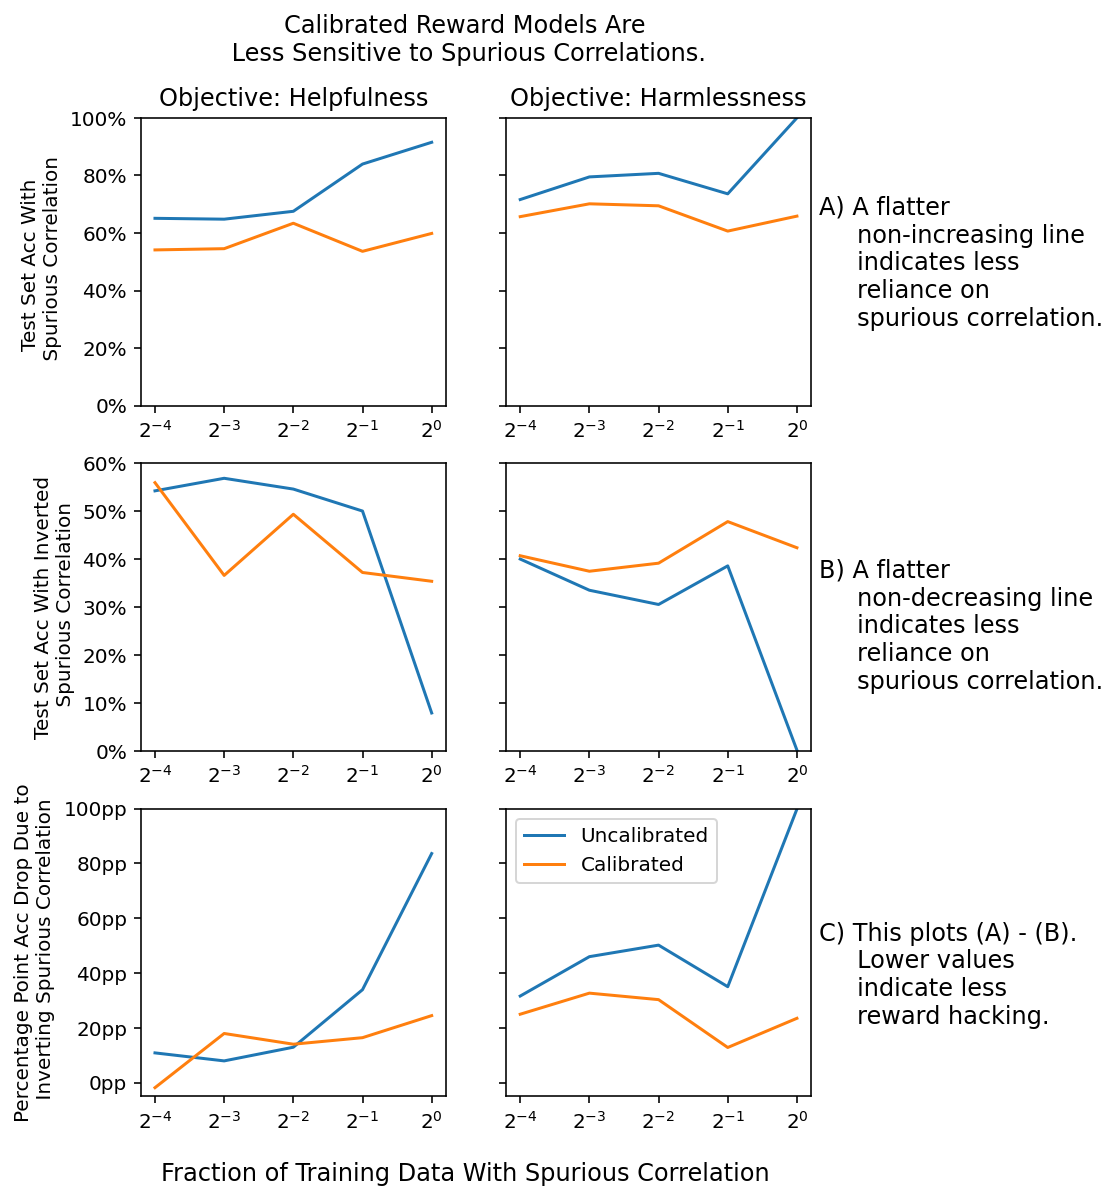
\includegraphics[width=0.65\columnwidth]{reward_hacking_fig.png}
    \caption{Calibrated reward models demonstrate robustness against reward hacking: We poisoned the training data by adding phrases to the preferred response to induce spurious correlations. When we evaluated against a test set where the correlations are inverted (phrase added to unpreferred models), calibrated models maintained higher accuracy than uncalibrated ones, demonstrating their reduced reliance on spurious correlations.}
    \label{fig:reward_hacking}
\end{figure}

\subsection{Gains are higher with more inference-time compute available} \label{sec:more_compute}
As can be seen, in \cref{fig:varying_n_winrate}, for $N=32$, we see better gains as compared to $N=2$ in both \bofn\ and \wofn\ win-rates on Anthropic helpfulness and harmlessness datasets. Thus, as more inference-time compute becomes available in the future, we find that \iapo can scale and further augment the performance gains. 

\begin{figure}
    \centering
    \begin{subfigure}{
    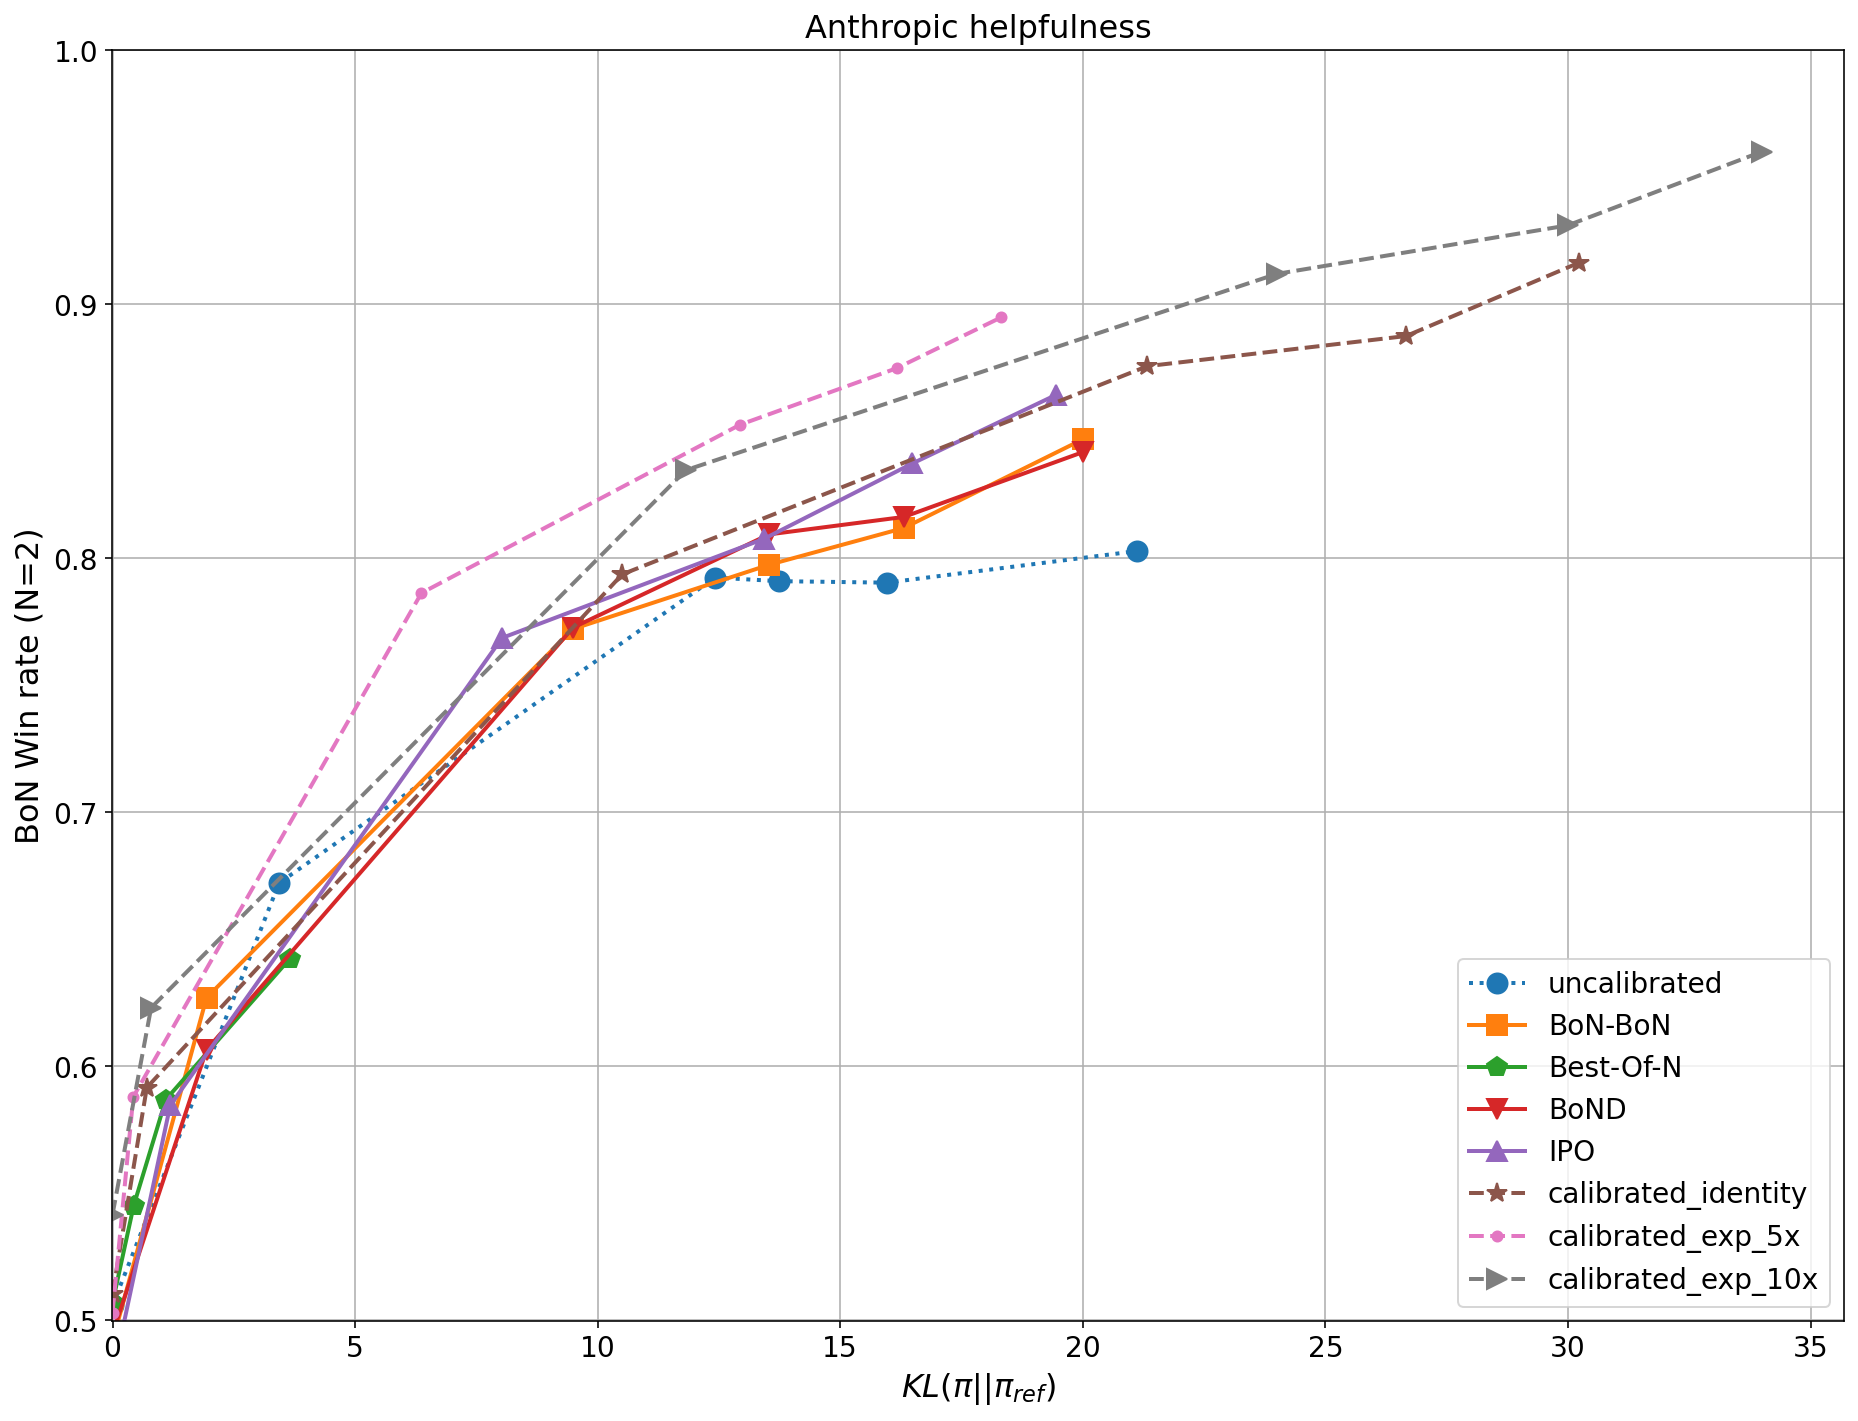
\includegraphics[width=0.45\columnwidth]{bon_win_rate_n_2.png}}
    \end{subfigure}
    \begin{subfigure}{
    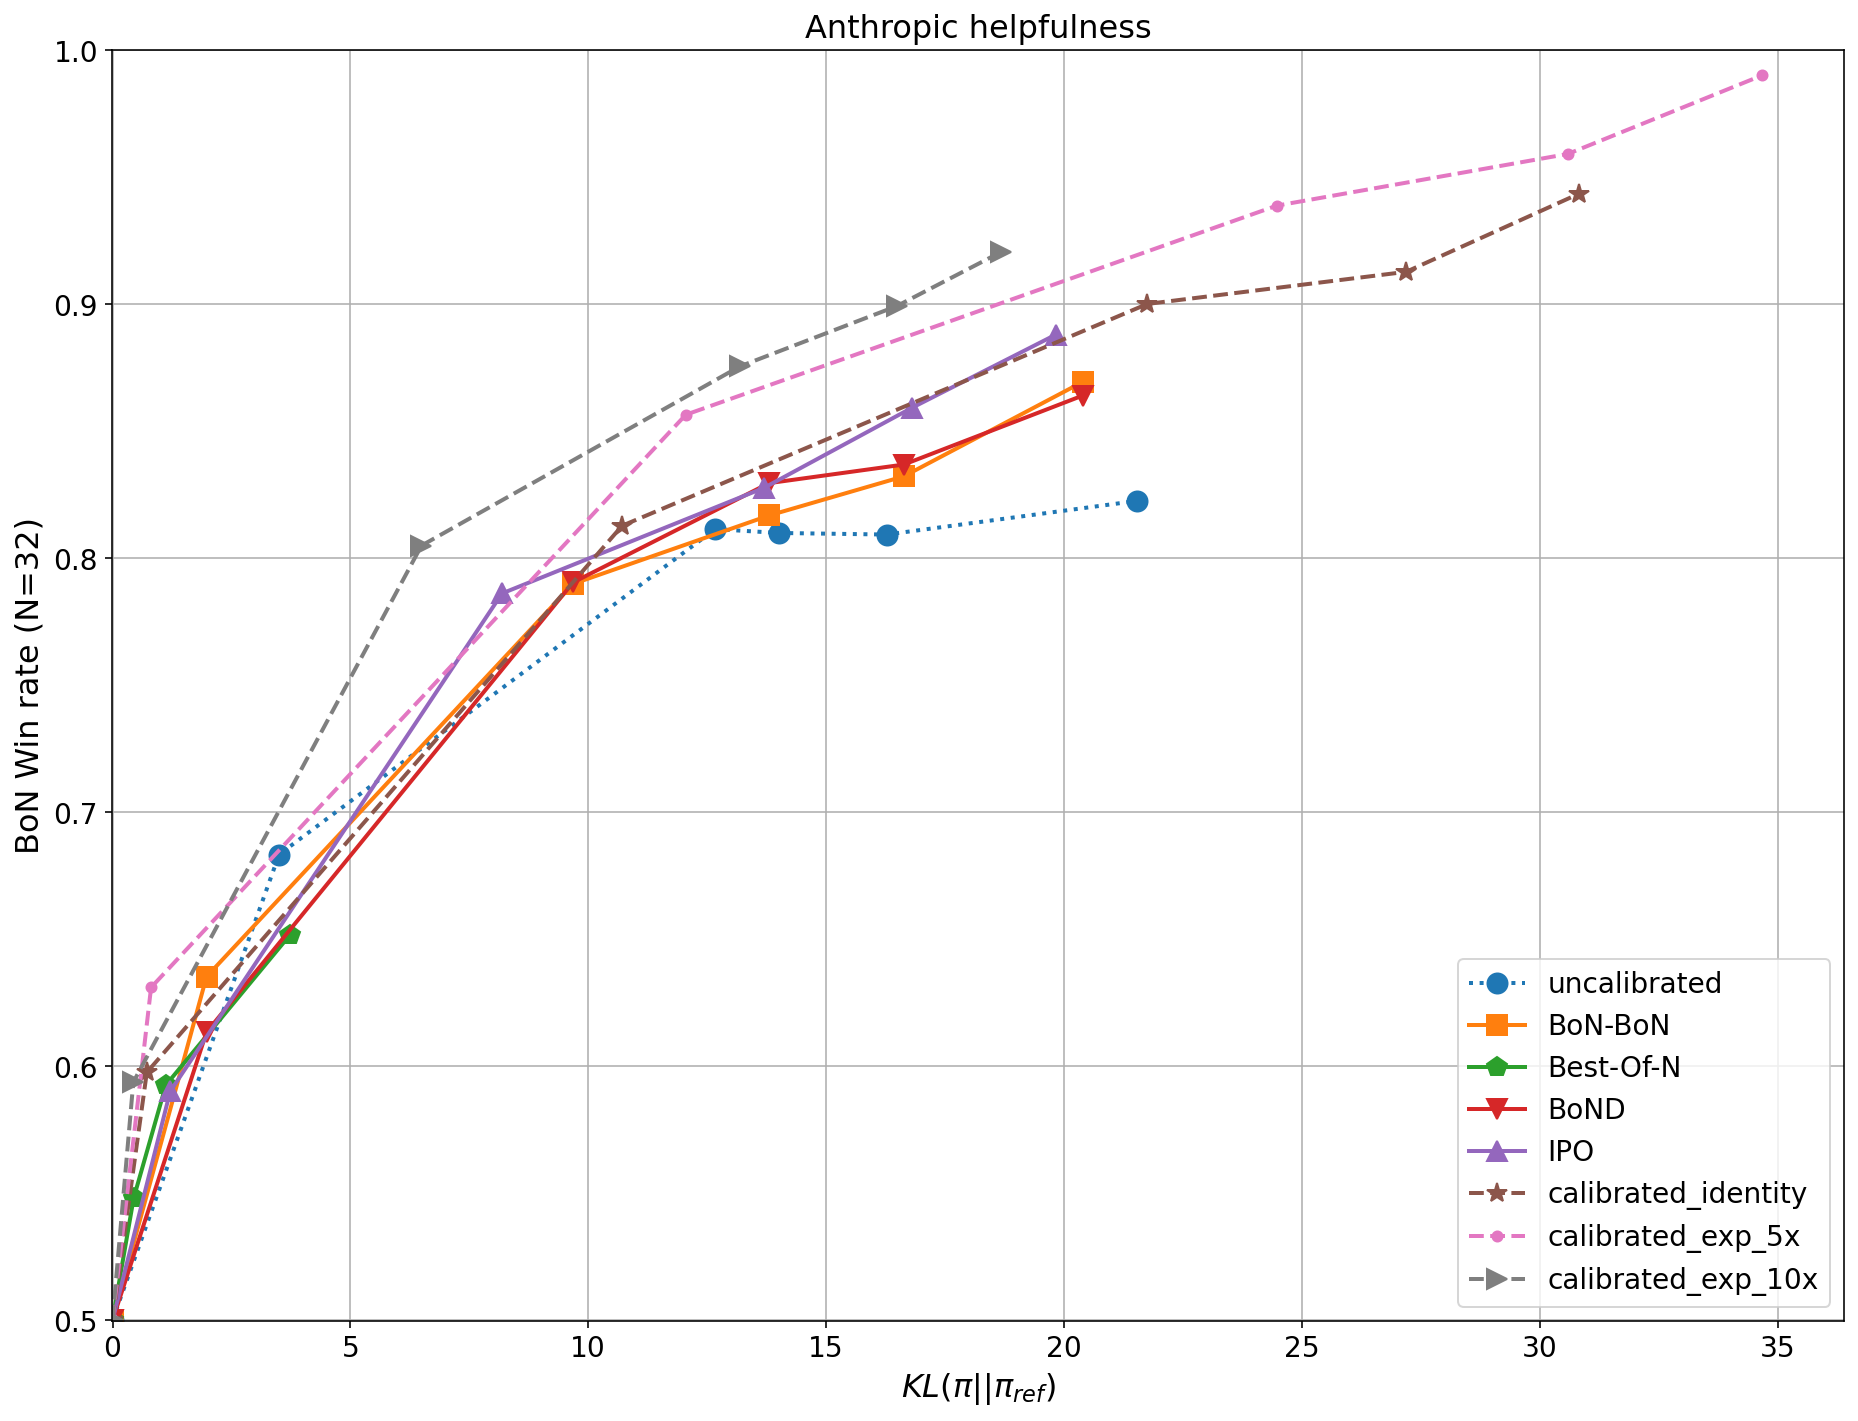
\includegraphics[width=0.45\columnwidth]{bon_win_rate_n_32.png}}
    \end{subfigure}
    \begin{subfigure}{
    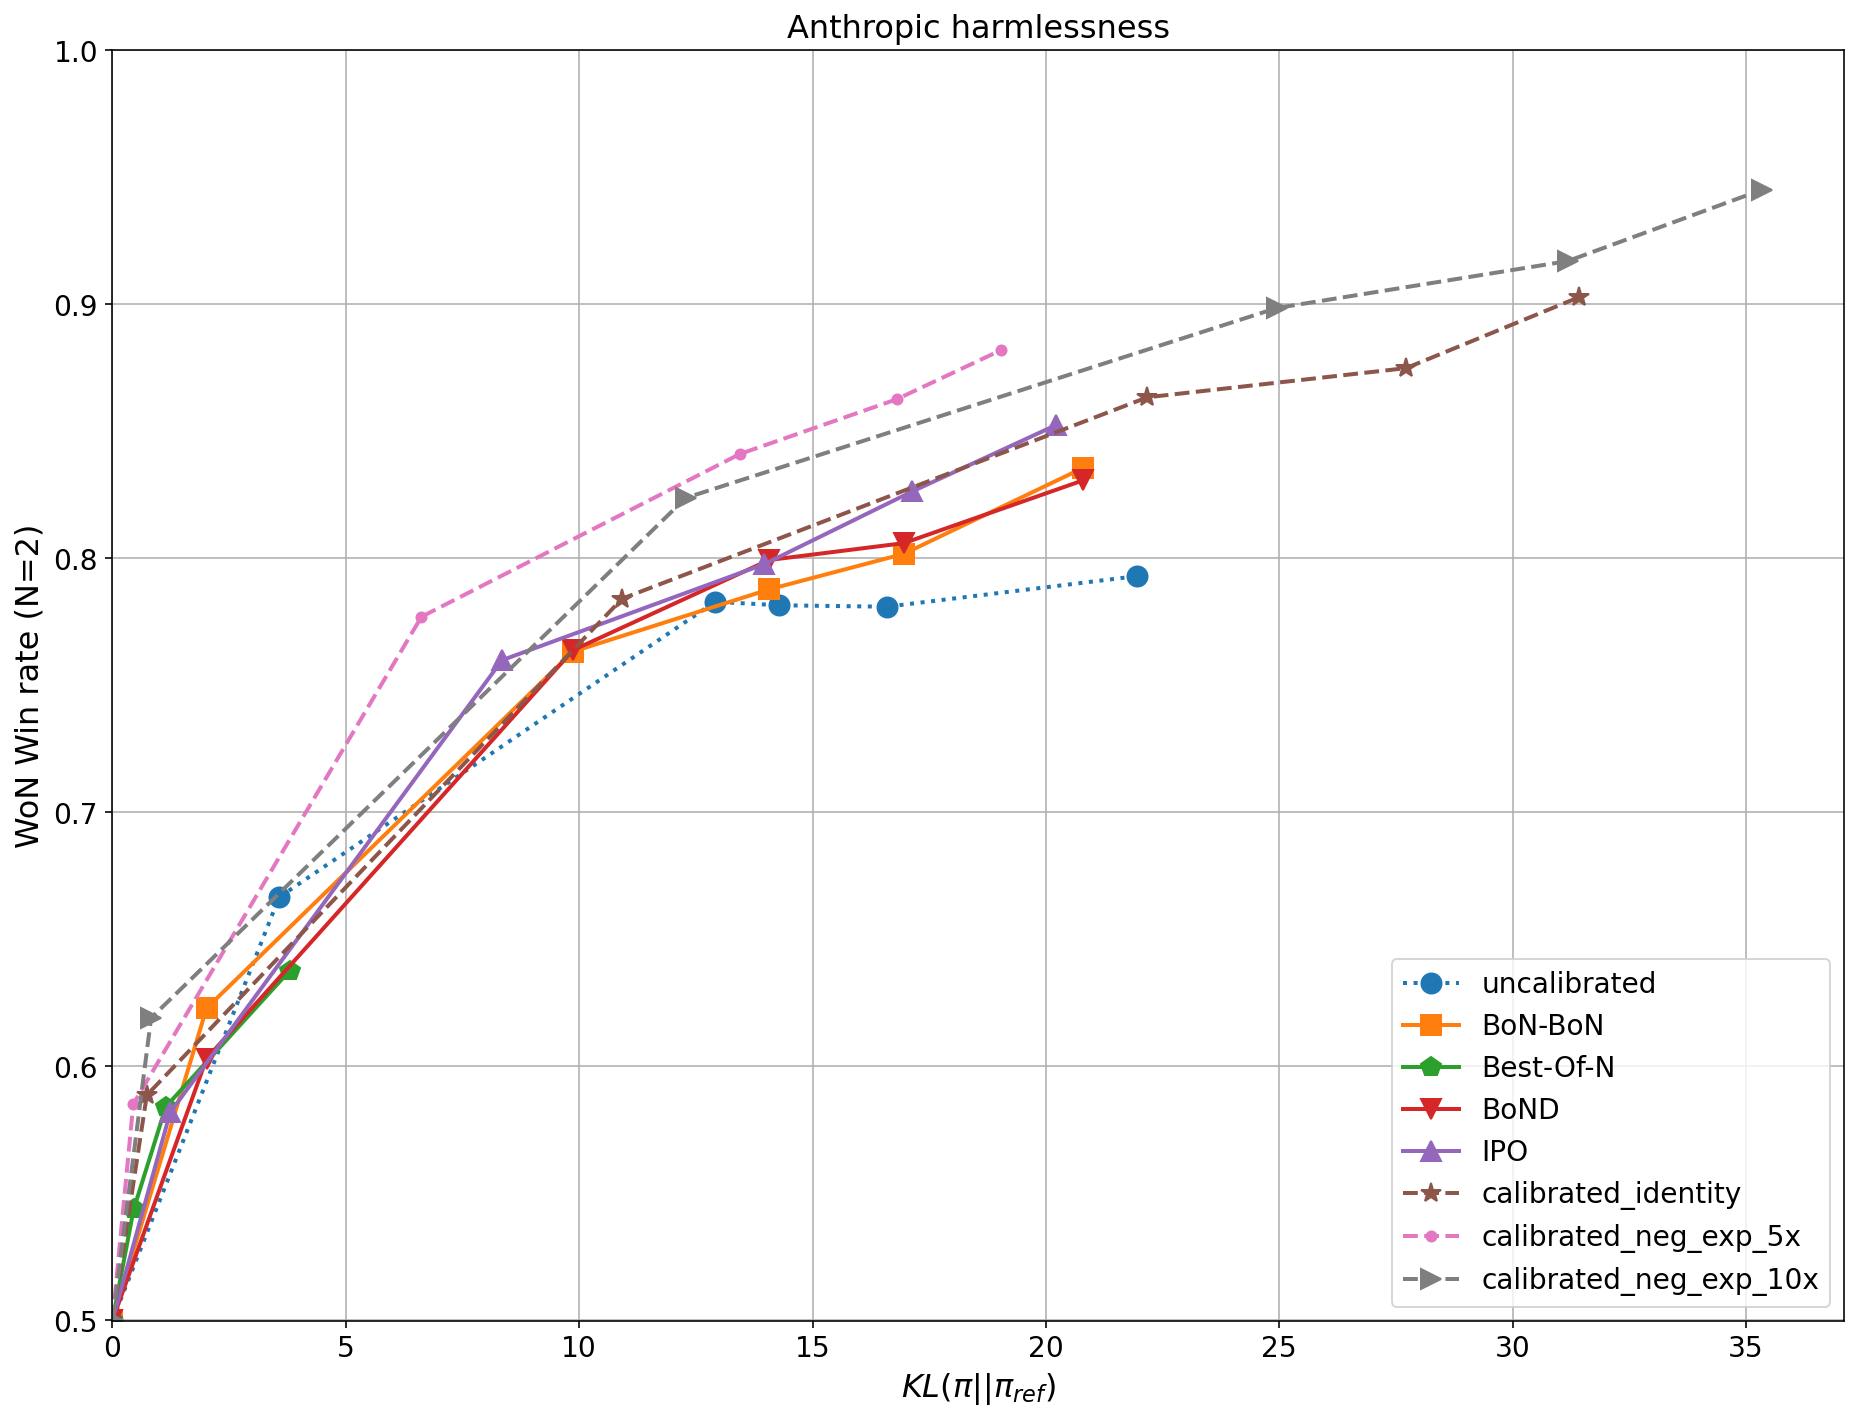
\includegraphics[width=0.45\columnwidth]{won_win_rate_n_2.png}}
    \end{subfigure}
    \begin{subfigure}{
    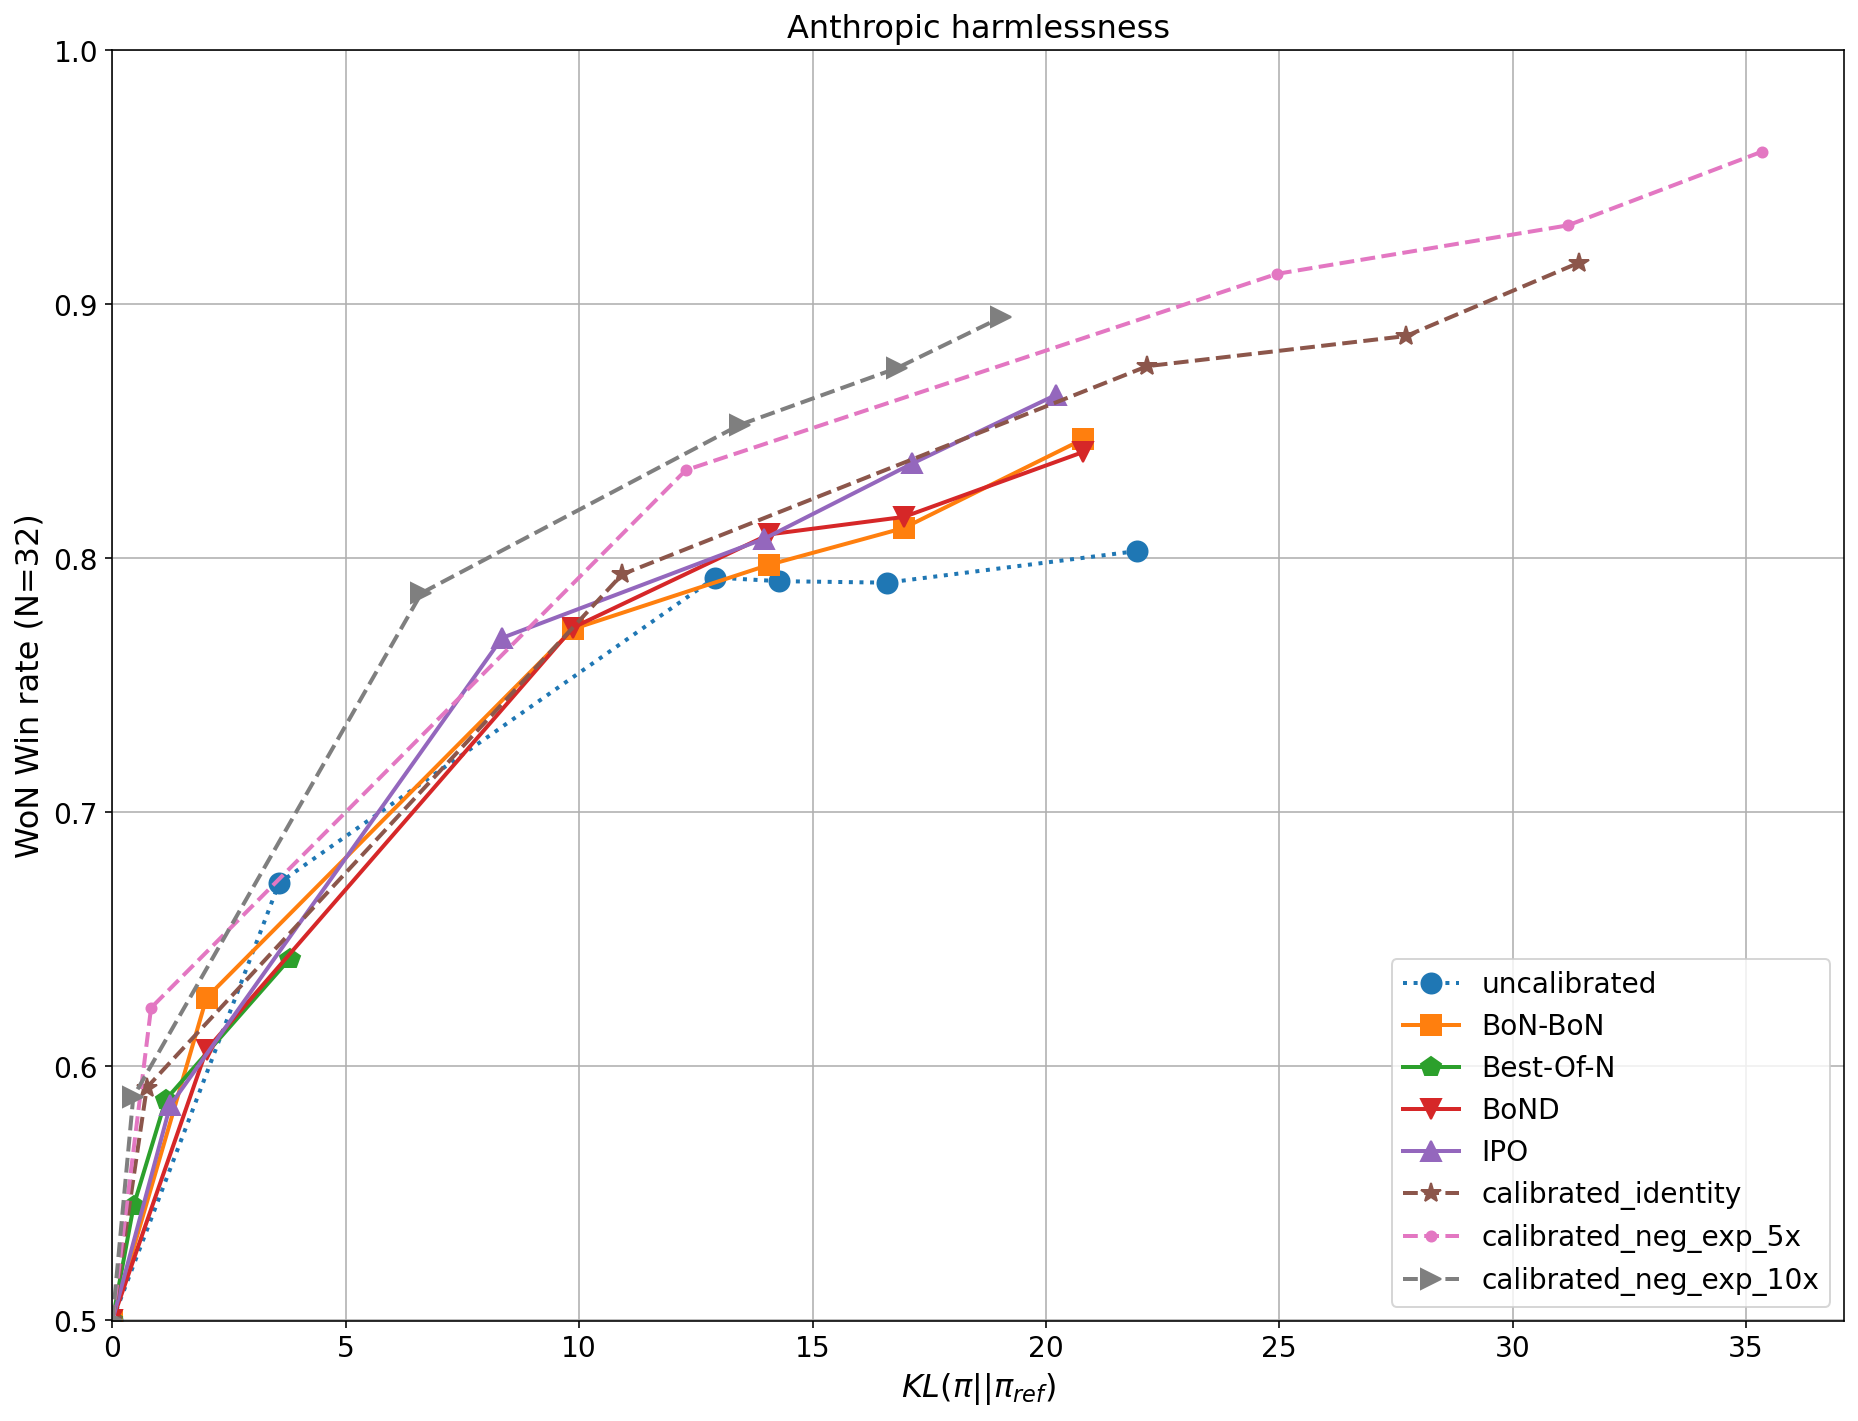
\includegraphics[width=0.45\columnwidth]{won_win_rate_n_32.png}}
    \end{subfigure}
    \caption{Higher N in \bofn\ and \wofn\ gives better gains in inference-time win rate-KL tradeoffs. The first row indicate the gains in \bofn helpfulness, and second on \wofn harmlessness for N=2,32.} 
    \label{fig:varying_n_winrate}
\end{figure}


%
%


%
%
%
%
%
%
%
%
%
%


%
%
%
%
%
%
%
%
%
%

%

%
%
%
%
%
%
%
%
%
%
%
%
%
%


%

%
%
%
%
%
%
%
%
%
%
%
%
%
%

%
%
%
%
%
%
%
%
%
%

%
%
%
%
%
%
%
%
%

%

%


%

%


%

%
%
%
%
    
%
    
%
    
%
%


%


%
%
%
%
%



%

%

%
\end{document}